\documentclass[pdftex,a4paper,halfparskip, article]{scrartcl}
% Andere Dokumentklassen: article, report, book, beamer, scrartcl, scrreprt, scrbook, beamer
% Prefix scr bedeuted aus dem KOMA-Script Paket, welches europäische Formatierungsstandards enthält
% Gebräuchliche Optionen sind: 11pt, 12pt, twoside, twocolumn, a4paper,...
\usepackage{ngerman} %Titel z.B. für Tabellen- und Inhaltsverzeichnis werden ins Deutsche übersetzt. Ausserdem Aktivierung der korrekten Silbentrennung

\usepackage{verbatim}
\usepackage[latin1, utf8]{inputenc} %Für das Erkennen von Umlauten

\usepackage[T1]{fontenc} %Font-Encodierung wird auf das T1-Format mit bis zu 256 (anstelle 128 im Default Fontencoder) umgeschaltet

\usepackage{hyperref}
\usepackage{graphicx}
\graphicspath{ {./images/} } 
\usepackage{color}

\title{Rapid Frontend Prototyping with Deep Learning} %Definition des Titels
\author{Simon Deussen}	%Definition des Autors
% \date{7.Nov.2010}

\begin{document}

\maketitle	

\begin{abstract}
Generierung von HTML/CSS Code für Websites aus Screenshots. Aufbauend auf dem Pix2Code Paper \cite{Beltramelli17}, ist diese Arbeit eine erweiterte Implementation mit mehr Elementen und damit komplexeren Websites. Dank Neuronaler Netze können Modelle erstellt werden, die selbständig valides HTML erzeugen. Durch automatisches Erstellen von Frontend-Code können Anwendungen wie diese rapide Entwicklungszyklen realisieren. 
\end{abstract}


\tableofcontents	% Erstellung des Inhaltsverzeichnisses
%\listoffigures   % Abbildungsverzeichnis
%\listoftables    % Tabellenverzeichnis
\section{Einleitung} 

Worin besteht der Nutzen automatisierter Code erstellen? Besonders im Bereich der Frontend-Entwicklung, bei der ein Team aus Leuten mit unterschiedlichen Fertigkeiten benötigt wird, kann es bei der Entwicklung zu Bottlenecks kommen. Im der klassischen Entwicklung sieht diese Zusammenarbeit folgendermaßen aus: \\
Ein Designer macht einen grafischen Entwurf, dieser wird vom Kunde abgenommen, dann geht er zu dem Entwickler, der nun zu aller erst Markup für den Content und anschließend das Design und die richtige Darstellung nach bauen muss. Für jede grafische Veränderung muss dieser Prozess wieder ausgeführt werden. Für die meisten Entwickler, ist die Markup und CSS-Erstellung der widrigste Part der ganzen Arbeit, da er recht zeit-aufwendig, repetitiv und langweilig ist.
Hier kommt es schließlich zu den Bottlenecks und Unzufriedenheit bei der Arbeit. Deswegen kann besonders ab der Schnittstelle zwischen Designern und Entwickler mit Automation viel gewonnen werden. Es gab bisher viele Ansätze diese Arbeit zu automatisieren, zum Beispiel durch Tools in dem man gleichzeitig Designen und den Markup exportieren kann. Leider sind diese Tools entweder nicht besonders gut darin, die Designs zu erstellen oder den Markup zu exportieren.

Eine Abhilfe soll diese Arbeit liefern: Sie ermöglicht, dass der Designer mit seinem bevorzugten Tools das Design entwickelt und der Entwickler mit einem Mausklick das fertige Markup bekommt. So kann sich der Entwickler vollends auf die Realisierung des Verhaltens und der Logik der Anwendung konzentrieren. 

\section{Ähnliche Arbeiten}

Diese Arbeit basiert auf dem Pix2Code Paper von Tony Beltramelli \cite{Beltramelli17}. Er war der erste der Code anhand von visuellen Input mit Neuronalen Netzwerken generieren hat. 
Anderen Ansätze wie DeepCoder \cite{DeepCoder16} benötigen komplizierte DSL als Input und schränken so die Benutzbarkeit stark ein. Visuelle Versuche mit Android-GUIs von Nguyen \cite{Nguyen15} benötigt ebenfalls unpraktische von Experten erstellte Heuristiken. Pix2Code ist so das erste Paper das einen allgemeinen Input hat, und daraus momentan drei verschiedene Targetsprachen hat. Zum einen kann es HTMl/CSS Code erstellen, zum anderen aber auch Android- und iOS-Markup. Siehe Original Code auf Github \cite{Beltramelli17Github}


\section{Motivation}

Computer genierte Programme werden die Zukunft der Software Entwicklung sein und diesen Bereich auch grundsätzlich verändern. Schon jetzt im Bereich der Cloud mit Serverless Computing und Lambdas, geht es oftmals bestehende Software-Teile zu verbinden. Diesen Trend, der für die Reduktion des Schreibens, mehr in die Richtung des Konfigurieren geht, sehe in Zukunft noch viel umfassender und allgegenwärtig. Es wird so weit gehen, dass man nicht nur wie hier in dieser Arbeit das Markup generiert sondern das aus einer Skizze sofort eine fertige Website gebaut wird, und man mit ein paar Klicks das nötige Verhalten einfach hinzufügen kann. 
Wobei dieser Trend nicht nur auf das Web bezogen ist. Ich denke das sich die Webtechnologien auch in der Desktop Umgebung durchsetzen.  Da Plattform unabhängig und sehr stark optimiert. Sehr einfach zu lernen, weit verbreitet. Zum Beispiel Electron \cite{electron} ermöglicht den einfachen Einsatz durch einen eingebettet Browser.
Daher kommt die Motivation diese Arbeit zu verfassen: Automation ist unumgänglich, deswegen sollte man diese am besten selber bauen und damit endlosen Entwicklern das Leben leichter machen.

\section{Benutzte Technologien}

In dem folgenden Abschnitt werden die benutzten Technologien beschrieben. Diese Erklärungen sind recht generell und gehen zunächst nicht auf die genaue Verwendung der Technologien in dem Projekt ein, dies wird aber im Abschnitt Überblick genauer beleuchtet.

\subsection{Neuronale Netzwerke}
Neuronale Netzwerke sind einfach zu benutzende Modelle, welche nicht-lineare Abhängigkeiten mit vielen latenten Variablen stochastisch abbilden können \cite{nnWebsite}. Im einfachen Sinne, sind sie gerichtete Graphen, deren Knoten oder Nodes aus ihren Inputs Werte errechnen und diese an die folgenden Nodes weitergeben. Hierbei werden zwischen 3 verschiedenen Arten von Nodes unterschieden:

\begin{description}
	\item[Input Nodes] Über diese Nodes bekommt das Netzwerke die Input Parameter.
	\item[Hidden Nodes] Nodes, welche das Netzwerke-interne Modell repräsentieren.
	\item[Output Nodes] Diese Nodes bilden die Repräsentation des Ergebnisses ab.
\end{description}

Nachdem die Node aus den Inputs einen Wert errechnet hat, geht dieser durch eine Aktivierungsfunktion. Diese Funktion stellt den Zusammenhang zwischen dem Input und dem Aktivitätslevel der Node her. Man unterscheidet zwischen folgenden Aktivitätsfunktionen

\begin{description}
	\item[Lineare Aktivitätsfunktion] Der einfachste Fall, linearer Zusammenhang zwischen Inputs und Output.
	\item[Lineare Aktivitätsfunktion mit Schwelle] Linearer Zusammenhang ab einem Schwellwert. Sehr nützlich um Rauschen herauszufiltern. Ein häufig genutzte Abhandlung davon:
	\begin{description}
		\item[ReLU] Hier werden nur der positive Werte weitergeleitet: \(f_x = x^+ = max(0,x) \)
	\end{description}
	\item[Binäre Schwellenfunktion] Nur zwei Zustände möglich: 0 oder 1 (oder auch -1 oder 1)
	\item[Sigmoide Aktivitätsfunktion] Benutzung entweder einer logistischen oder Tangens-Hyperbolicus Funktion. Diese Funktionen gehen bei sehr großen Werten gegen 1 und bei sehr negativen Werten gegen 0 (logistische Funktion) oder -1 (Tangens-Hyperbolicus Funktion). Diese Funktion bietet den Vorteil das sie das Aktivitätlevel begrenzt.
\end{description} 

Jede der Nodes hat eine bestimmte Anzahl an Verbindungen, diese hängt von der Art der Nodes und deren Zweck ab. Wichtig ist jedoch, das jede Node mit mehreren anderen Nodes verbunden ist, dies soll heißen, den Output mehrerer Nodes als Input zu bekommen und den eigenen Output als Input für die folgenden Nodes weiterzuleiten. Die Stärke der Abhängigkeit zwischen zwei Nodes wird als Gewicht ausgedrückt. Jede Verbindung in einem Neuronalen Netzwerk hat ein Gewicht, welches mit dem Output der vorangegangen Node multipliziert wird bevor es als Input weiter verwendet wird.

Das Netzwerk-interne Modell wird in diesen Gewichten abgespeichert. Es repräsentiert also das Wissen, dass durch das Training entstanden ist.

Das Training eines Netzwerkes, ist das schrittweise Anpassen der Gewichte bis es ein gutes Modell des Problems gelernt hat. Die Stärke von Neuronalen Netzen liegt darin, aus großen Mengen von Daten Gesetzmäßigkeiten oder Patterns zu erkennen. Ein einfaches Beispiel ist die Objekterkennung. Wenn ein Netzwerk Alltagsgegenstände erkennen soll, lernt es die Pixelgruppen welche ein Tisch von einem Bett unterscheiden. Damit dies funktioniert braucht man eine große Menge an Daten. Zunächst wird das Training in zwei verschieden Arten unterteilt: 

\begin{description}
	\item[Supervised learning] Innerhalb des Trainingsdatensets, hat jeder Datensatz einen vorgegeben Output Label. Zum Beispiel ein Bild von einem Auto ist auch so gekennzeichnet. Nun werden so lange die Gewichte des Netzwerkes optimiert, bis ein jeweiliger Input auch den richtigen Output erzeugt.
	\item[Unupervised learning] Hier hat das Trainingsdatenset keine Label. Die Gewichtsveränderungen erfolgen im Bezug zur der Ähnlichkeit von Inputs. Das soll heißen, wenn es viele verschiedene Bilder bekommt, werden Bilder mit ähnlichen Inhalten eine hohe Nähe aufweisen, ein Bild von einem PKW wird näher an dem Bild von einem LKW sein als an dem Bild von einem Apfel.
\end{description}

\subsection{Convolutional Neural Network - CNN}

CNN sind Tiefe Neuronale Netzwerke mit einer bestimmten Architektur und spezialisiert auf die Verarbeitung von Bildern. Da man die Anwendungsdomäne eingeschränkt hat, kann man bestimmte Annahmen treffen, welche die Anzahl der Verbindungen und damit Rechenoperationen verringert und somit das Netz effektiver macht. Um aus Bildern, Informationen zu gewinnen, müssen die Ebenen des Netzwerkes nicht vollständig verbunden sein. Stattdessen werden Filter (Convolutions) und Sub-Sampling genutzt \cite{colahsBlogCnn}. Filter sind kleine Matrizen, die bestimmte Features entdecken, zum Beispiel Kanten mit bestimmter Ausrichtung. Durch das Erlernen der Filter im Training kann das Netzwerk aus den Pixel Werten, schrittweise abstraktere Features errechnen. Diese gehen von einfachen Kanten, zu komplexeren Umrissen, und schließlich zu vollständigen Teil-Objekten . Zum Beispiel werden aus vielen Kanten ein Kreis, dann kommen noch mehr dazu bis eine Feautere Map ein Auge abbildet. 
Aus dem Auge und der biologischen Signal Verarbeitung ist diese Architektur inspiriert \cite{Hubel68}. Einzelne Neuronen des celebralen Kortex reagieren auf Reize nur in einem beschränkten Bereich. Da diese Bereiche leicht überlappen können so diese Neuronen den gesamten Sichtbereich erkennen. 

\begin{figure}[h]
\centering
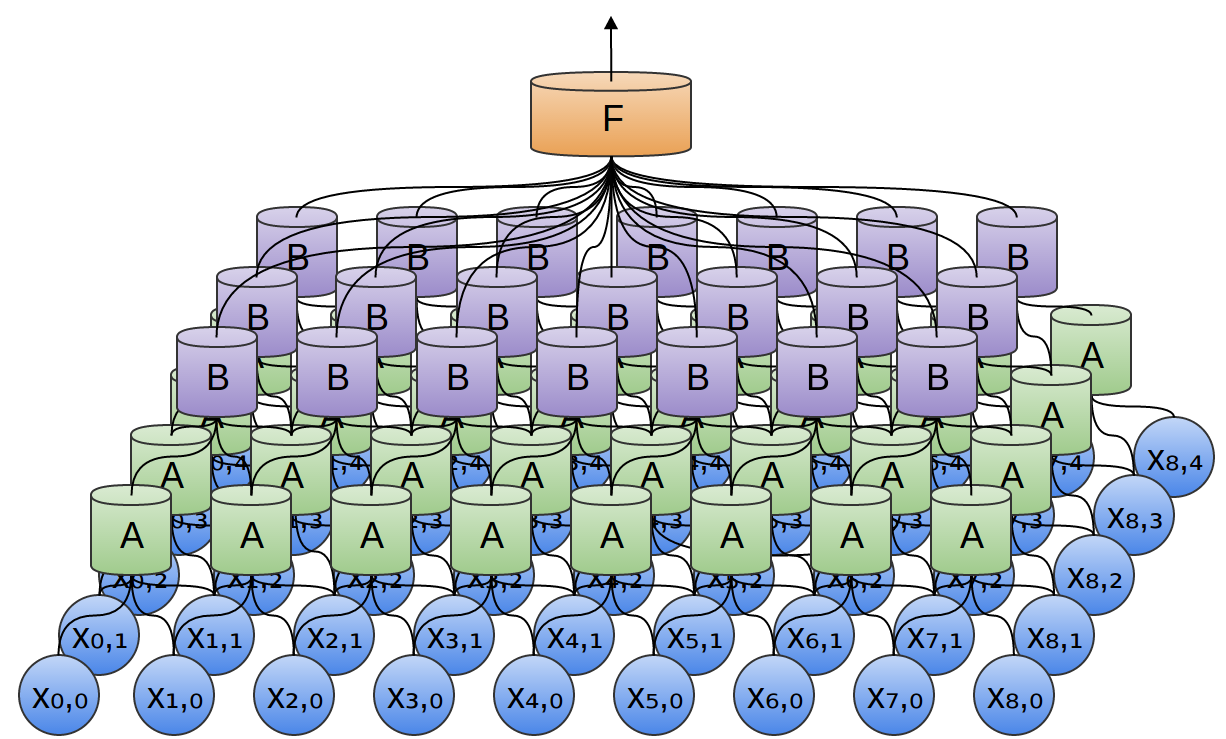
\includegraphics[width=0.5\textwidth]{colah_cnn}
\caption{CNN von \url{http://colah.github.io/}}
\label{fig:colah-cnn}
\end{figure}


In Neuronalen Netzen sind Fully-Connected-Layer die Ebenen mit den meisten Verbindungen. Bei Betrachtung der Abbildung~\ref{fig:colah-cnn}, würde eine Fully-Connected-Layer insgesamt $ n = 9^2 * 5^2 = 2025$ Verbindungen zwischen $x_{i, j}$ und $A$ benötigen. Stattdessen benötigen die Convolutional-Ebene mit einem Kernel von $2*2$ nur $n = 8 * 5 *4 = 128$ Verbindungen. Abgesehen von den Einsparung der Verbindungen, hat ein CNN viele verschiedene Kernel, welche sich pro jeweils die gelernten Gewichte teilen \cite{colahsBlogCnn}. Für jeden Kernel $A$ in der Abbildung werden die gleichen 4 Gewichte gebraucht. Diese Gewichte werden während dem Training gelernt und bilden dann ein bestimmtes Feature der Input-Daten ab, wie oben beschrieben.

\begin{figure}
\centering
\begin{minipage}{.5\textwidth}
  \centering
  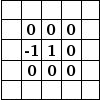
\includegraphics[width=.3\linewidth]{gimp_doku_edges_kernel}
\end{minipage}%
\begin{minipage}{.5\textwidth}
  \centering
  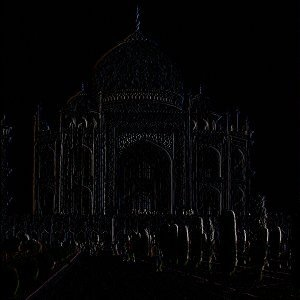
\includegraphics[width=.8\linewidth]{gimp_doku_edges}
  \end{minipage}
\captionof{figure}{Beispiel Kernel aus der Gimp-Dokumentation \cite{gimpdoku}}
  \label{fig:kernel}
\end{figure}

Die Operationen die Kernel auf einem Input ausführen, ist in Abbildung~\ref{fig:kernel} visualisiert. Hier wird durch eine einfache Convolution eine Repräsentation des Inputs gebildet, in der nur vertikale Kanten enthalten sind. Wenn nun ein Kernel mit einer derartigen Operation in Netzwerk aktiviert wird, teilt dieser dem Rest des Netzwerkes mit, dass hier eine vertikale Kante in Input ist.

Durch das Kopieren der Kernel und der geringeren Verbindungsanzahl sind nun sehr große und sehr tiefe Modelle möglich. In 2012, haben Krizhevsky et al. die Welt der Bildklassifizierung mit ihrem Paper und den darin vorgestellten Modell revolutioniert \cite{ImageNetOriginal}. Ihr tiefes, convolutional Neural Network konnte insgesamt 1000 Klassen unterscheiden mit einer Genauigkeit von 63\%. Deren Ergebnisse waren der Anfang einer neuen Art von Bildklassifizierung, und es folgten viele weitere Paper die auf deren Erfolg aufbauend, CNNs tief in der Computer Vision verankerten \cite{colahsBlogCnn}.

\subsection{Recurrent Neural Network - RNN}

RNNs sind eine Erweiterung der klassischen Feedforward Netze, die im Stande sind, Input-Sequenzen mit verschiedener Länge zu verarbeiten \cite{paperGRUComparison}. Die RNN schaffen dies, in dem sie einen inneren Zustand haben, dessen Aktivierungen von vorherigen Inputs abhängig sind.
RNNs haben Verbindungen zu Neuronen der selben oder vorhergehenden Schichten und können dadurch Inputs durch das gesamte Netz durchgeben. 

\begin{figure}[h]
\centering
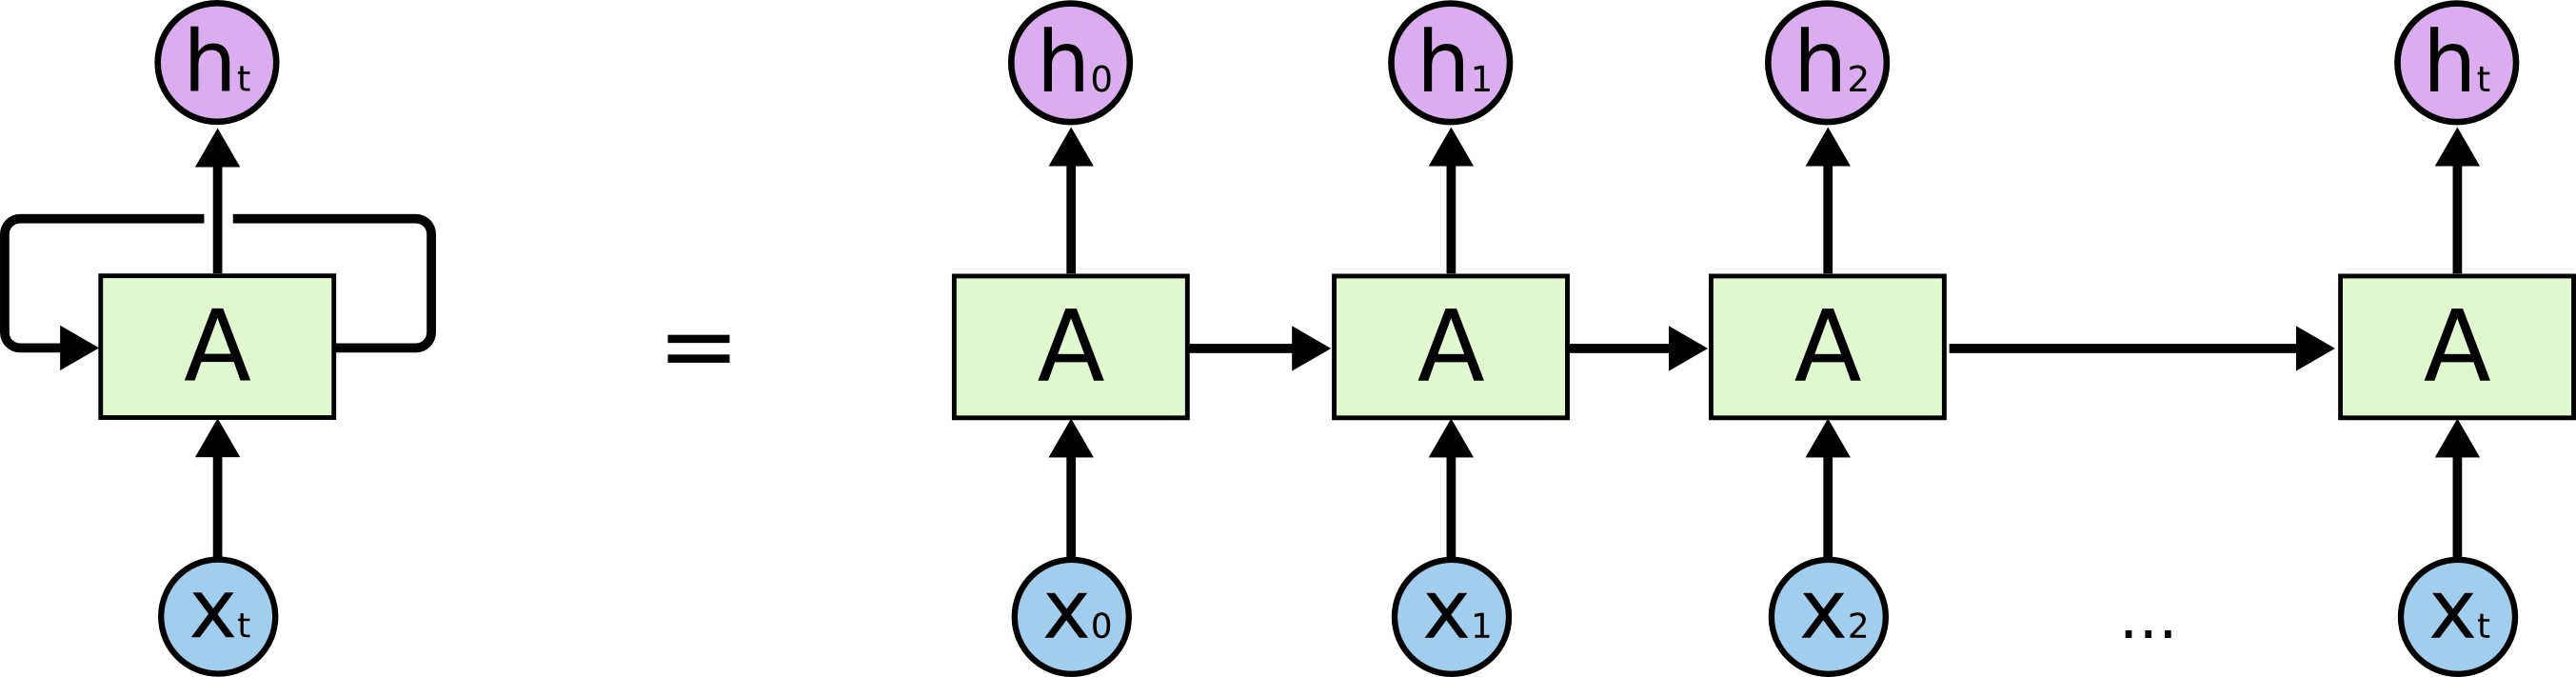
\includegraphics[width=0.5\textwidth]{colah_rnn}
\caption{RNN von \url{http://colah.github.io/}}
\end{figure}

Wie auf der Abbildung zu sehen ist, ähnelt der Verbund der Rekurrenten Einheiten einer Liste. Damit ist diese Art Neuraler Netzwerke besonders gut geeignet sequentielle Daten abzuarbeiten \cite{colahsBlogLSTM}. Listen, Sprachsynthese und Maschinelle Übersetzungen sind Bereiche wofür RNNs gut geignet sind.



\subsubsection{Long short-term Memory - LSTM}

Ein LSTM ist eine bestimmte Form der RNNs. Ein RNN kann durch dessen starre Struktur immer nur eine bestimmte Anzahl von Schritten abspeichern. Die Schrittanzahl hängt davon ab, wie viele RNN-Units mit einander verkettet sind. Sobald mal jedoch einen sehr weiten Kontext benötigt, zum Beispiel bei der Analyse von Texten oder der maschinellen Übersetzung, stößt diese starre Struktur an ihre Grenzen. Ein LSTM ist so gebaut, dass es die einzelnen Units selber entscheiden können, welche Daten weiter beibehalten oder vergessen werden. Durch die dynamische Speicherverwaltung, kann es auf der einen Seite sich bestimmte Informationen länger speichern, auf der anderen, kurzfristig benötigte Daten verarbeiten und dann wieder vergessen. Während des Trainings eines LSTMs, erlernt dieses auch das Speichern und Löschen. Dadurch kann es sehr viel effizienter als reine RNNs Daten mit temporaler Dimension auswerten. Fast jeder Erfolg, der mit RNNs erzielt wurde, ist auf LSTMs zurückzuführen \cite{colahsBlogLSTM}. 

Eingeführt wurde das LSTM von Hochreiter und Schmidhuber im Jahr 1997 \cite{LSTM_orig}. Seit dem wurden viele Variationen davon getestet, verworfen und verbessert. In dieser Arbeit, wird mit dem Begriff LSTM diese Original Spezifikation gemeint.

\begin{figure}[h]
\centering
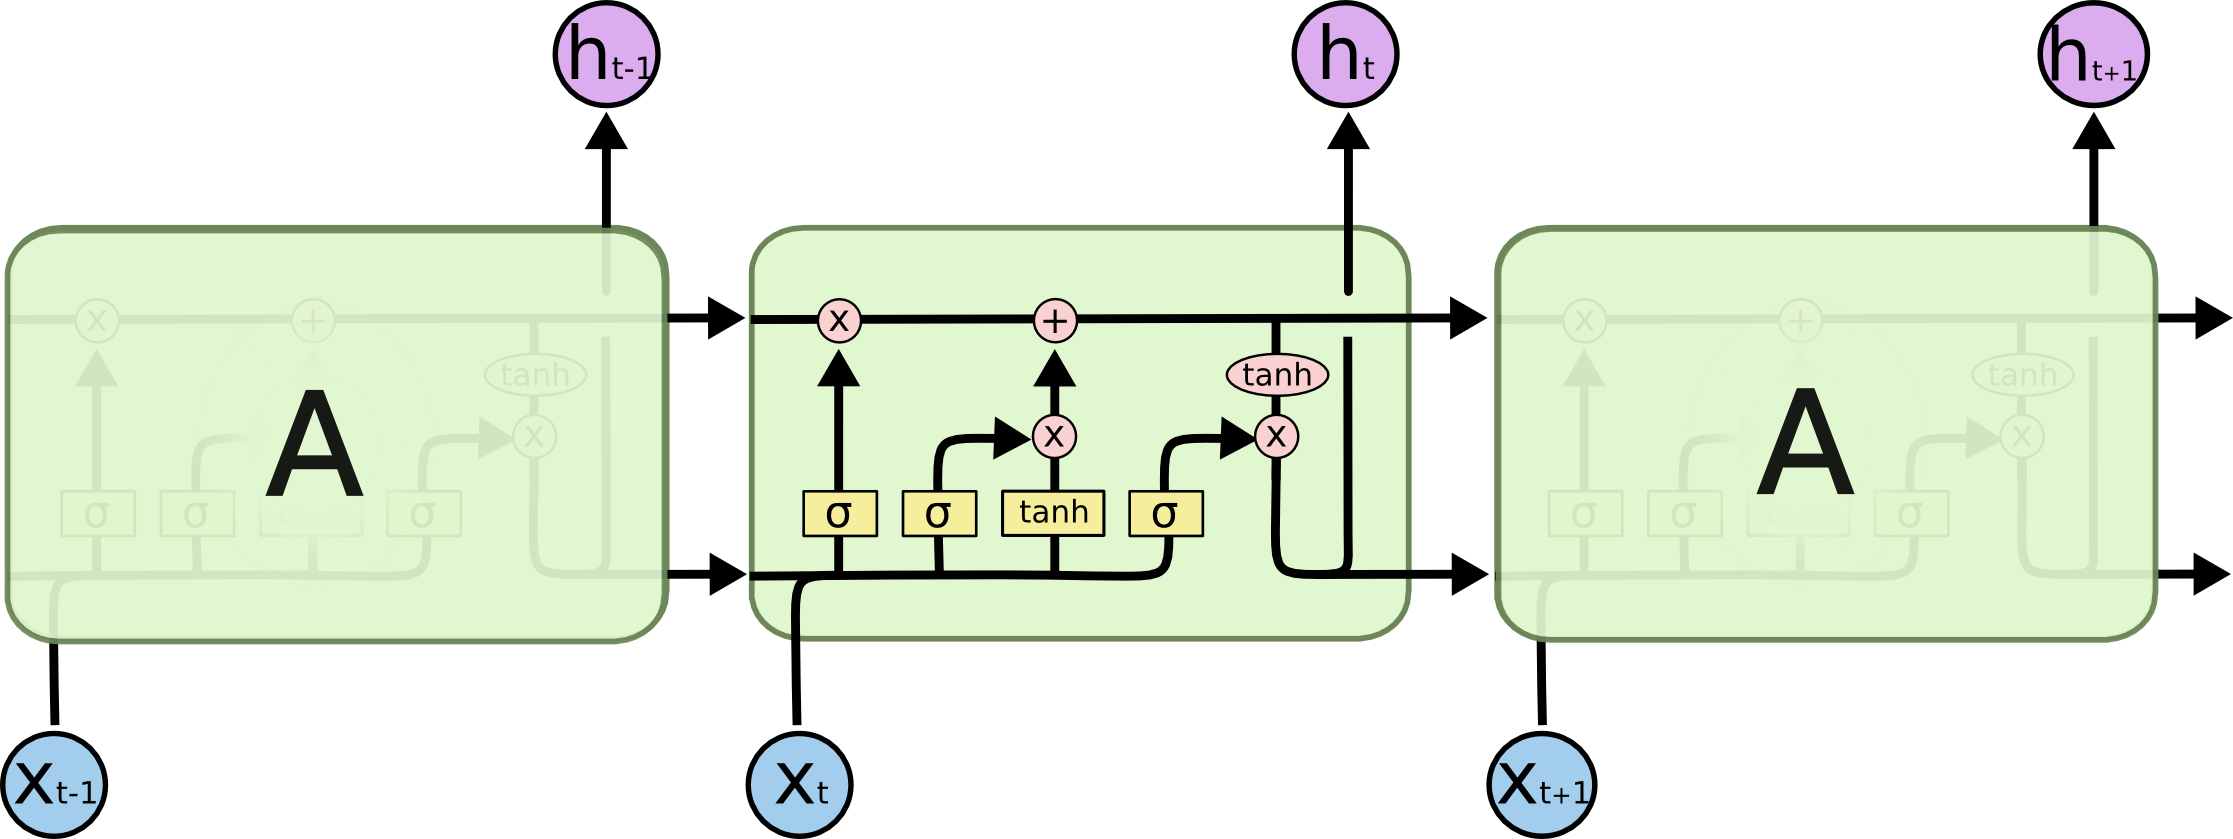
\includegraphics[width=0.5\textwidth]{colah_lstm}
\caption{LSTM von \url{http://colah.github.io/}}
\end{figure}

Eine LSTM-Unit teilt sich mit allen anderen LSTM-Units des Netzwerkes einen Cell-State, in der Abbildung die obere, horzontale Linie. Jede Unit kann diesen auf zwei Arten verändern, mit einem \texttt{forget}-Gate werden Informationen vergessen, mit einem \texttt{add}-Gate Informationen hinzugefügt. Schließlich berechnet jede Unit einen eigenen Hidden-State anhand des Inputs, des geteilten Cell-States und dem Hidden-State vorangegangener Units.


\subsubsection{Gated Recurrent Unit - GRU}

Die GRU, ist eine Abwandlung des klassischen LSTM. Die Architektur wurde 2014 von Kyunghyun Cho et al. eingeführt \cite{DBLP:journals/corr/ChoMGBSB14}. Was diese Variante ausmacht, ist eine Zussammenführung des \texttt{forget}- und \texttt{add}-Gates, sowie das Weglassen des Cell-States. Dadurch hat es weniger Parameter als die klassische Variante.
\begin{figure}[h]
\centering
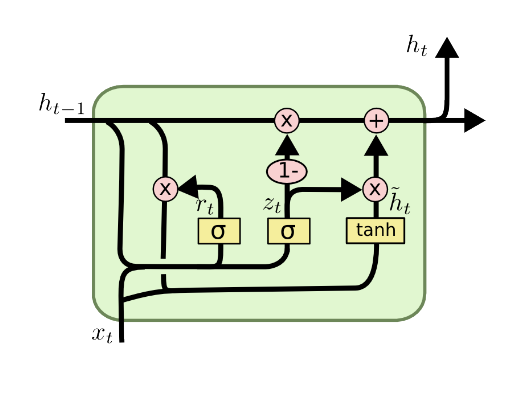
\includegraphics[width=0.3\textwidth]{colah_gru_small}
\caption{GRU von \url{http://colah.github.io/}}
\end{figure}
Trotz der geringeren Anzahl an Parameter, ist die Performance ähnlich der klassische Variante\cite{lstmSearchSpace}, trainiert aber schneller, da weniger optimiert werden muss. 


\subsection{Training}

Als Training wird der Prozess bezeichnet, während dem ein Neurales Netzwerk Wissen aus vorliegenden Daten extrahiert. Genau dieser Vorgang sorgt für den großen Erfolg von Neuralen Netzen. Anders als bei herkömmlichen Statistischen Methoden können NNs aus riesigen Datenmengen Patterns und Sachverhältnisse lernen. Damit dies funktioniert, muss eine Kostenfunktion gebildet werden können, anhand bestimmt wird, wie weit das genutzte Modell von der Optimalen Lösung entfernt ist. Anhand diesem Abstand können die Parameter des gewählten Modells angepasst werden um dem Optimum näher zu kommen.

\subsubsection{Overfitting}
	
Overfitting tritt ein, wenn das Modell zu Komplex für den gewählten Task ist, und deswegen die Trainingsdaten auswendig lernt. Somit wird es sehr gute Ergebnisse auf dem Trainingsset zeigen, sobald es aber Daten bekommt, die es nicht kennt, wird die Performance abstürzen da es nicht Verallgemeinern kann.

\subsubsection{Stochastig Gradient Descent - SGD}

SGD ist eine iterative Methode um ableitbare Funktionen und Modelle zu optimieren. Um ein Modell zu optimieren, wird eine Verlustfunktion benötigt. Diese zeigt den Schaden an, der entsteht wenn das Modell mit falschen Parametern Entscheidungen trifft. Um die richtigen Parameter während des Trainings zu finden, muss diese Verlustfunktion minimiert werden.
Bei SGD werden durch zufällige Samples des Trainingssets, Näherungen an den Gradienten gebildet, die dann wiederum genutzt werden um die Parameter zu optimieren. Nach mehreren Durchläufen durch das Trainingsset wird ein Set an Parameters gefunden, die ein Minimum der Verlustfunktion bilden \cite{walkSGD}. 


\begin{description}
	\item[RMSprob] Eine Variante des SGD, die sich besonders gut eignet um RNNs zu optimieren \cite{kerasDocRMSprob}. Diese wird in der Arbeit genutzt.
\end{description}

\subsubsection{Dropout}

Dropout ist eine Technik, die genutzt wird um Overfitting zu vermeiden. Während des Trainings werden zufällig Nodes sowie ihre Eingangs- und Ausgangsverbindungen aus dem Netzwerk entfernt \cite{JMLR:v15:srivastava14a}.


\subsection{Sampling}
Während dem Sampling, wird ein fertig trainiertes Neurales Netzwerk genutzt um aus Daten Schlussfolgerungen abzuleiten. In dem Fall dieser Arbeit, wird probiert aus einem Screenshot, eine deutungsvolle DSL-Sequenz zu erstellen.

\subsection{Keras}
Um die in dieser Arbeit genutzten Tiefen Neuronalen Netzwerke zu definieren wir das Framework Keras genutzt. Es ist eine Library die es sehr einfach macht Neuronale Netzwerke zu erstellen und verwalten. Es selber verwaltet nur die Definition von Modellen, die eigentlichen Berechnungen werden im Backend getätigt, von Theano, Tensorflow oder CNTK. So ermöglich es schnelles experimentieren mit wenig Overhead und keinen Boilerplate-Code. 

\subsection{Domain-specific language - DSL}

Eine Programmiersprache, die auf ein einzelne Problem-Domäne spezialisiert ist, wird DSL genannt. Im Gegensatz zur DSL steht die General Purpose Language, welches ein Programmiersprache ist, die sehr breit, für viele verschiedene Anwendungen, benutzt werden kann. Die Trennung zwischen DSL und GPL ist nicht immer klar, es kann zum Beispiel Teile einer Sprache geben die hoch spezialisiert für eine bestimmte Aufgabe sind, aber andere Teile von ihr können allgemeinere Aufgaben lösen. Auch historisch bedingt kann sich die Einordnung einer Sprache ändern. JavaScript wurde ursprünglich für ganz einfache Steuerung von Websites eingeführt, kann aber inzwischen für alles mögliche eingesetzt werden - vom Trainieren von CNNs im Browser, zu klassischen Backend-Jobs. 
In dieser Arbeit, wird eine hochspezialisierte, eigens erstellte Sprache aus Token, die eine Kombination aus HTML und CSS sind, benutzt.

\subsubsection{Hypertext Markup Language - HTML}
HTML ist die Standard Programmiersprache um Websites zu erstellen. Mit einzelnen HTML Elementen beschreibt es den semantischen Zusammenhang des Contents von Websites.

\subsubsection{Cascading Style Sheets - CSS}
CSS beschreibt die Präsentation, also das Aussehen, des Content einer Markup-Language (zum Beispiel HTML). Klassische Inhalte, sind Farben, Positionen und Effekte von User Interface Elementen.
 

\section{Rapid Frontend Prototyping - Überblick}

RFP ist ein Tool. welches aus einfachen GUI-Screenshots HTML/CSS Markup erzeugen kann. Dafür lernt ein System aus Neuralen Netzwerken eine einfache Token Sprache / DSL. Jedes Wort dieser Sprache hat zugehörigen HTML/CSS Markup, wodurch es nach Erstellung der Tokens einfach in diese Sprache kompiliert werden kann.

Um den Code für die Website Screenshots zu generieren, wird ein Modell bestehend aus 2 LSTMs und einem CNN erstellt. Das hier benutzte Modell ist eine Abwandlung des im Original Paper verwendeten Modells. Da die neue DSL komplexer als die im Original Paper\cite{Beltramelli17} ist, musste sowohl das CNN als auch die LSTMs verändert werden. 

Von einem Computer abgespeicherte Bilder sind ein denkbar schlechtes Format um aus den Rohdaten auf Inhalte zuschließen. Zu Grunde liegen ist jedes Bild ein oder mehrere Matrizen deren einzelne Elemente einem Pixel zugeordnet werden. Um aus diesem Zahlenwerten Schlussfolgerungen zu schließen, müssen diese in mehreren Schritten abstrahiert werden um zu einem bedeutungsvollem Datenmodell zu kommen. Hierfür wird ein CNN genutzt. Dieses verarbeitet das gegebene Input-Bild und erstellt eine niedrig-dimensionalere Repräsentation. Die Architektur des CNN ist recht simple und angelehnt an VGGNet von Simonyan and Zisserman. 

\section{Daten Synthese}

Da im Zuge dieser Arbeit eine Erweiterung der DSL des Original Papers implementiert wurde, ist es erforderlich, neue Trainingsdaten zu synthetisieren. Das DataCreationTool ist ein Programm, welches nach vorgegebenen Regeln einen Token-Baum erzeugt und diesen anschließend abspeichert. Dieser Token-Baum hat immer einen body-Token als Wurzel und der gesamten Inhalt liegt als dessen Kinder vor. Dafür wurde eine Helfer Klasse geschrieben, die ein Element in dem Token Baum abbildet. Diese kann zum einen Parameter wie den Token-Name, Inhalt und Kinder speichern, zum anderen enthält sie Funktionen zum Konvertieren des Baumes zu einer String-Repräsentation sowie zum Rendering nach HTML/CSS. 

\subsection{Generieren der Token-Bäume}
Die Token-Bäume werden in der Datei \texttt{createAllTokens.py} generiert. Diese Datei erzeugt alle möglichen Token-Kombination anhand der folgenden Regeln:

\subsubsection{Gramatik}

\begin{equation}
start \rightarrow [H,C]
\end{equation}

\begin{equation}
H \rightarrow [Ml | Mr | S]
\end{equation}
\begin{equation}
Ml \rightarrow  [ logoLeft, buttonWhite | logoLeft, buttonWhite, buttonWhite | ...]
\end{equation}
\begin{equation}
Mr \rightarrow [buttonWhite, logoRight | buttonWhite, buttonWhite, logoRight | ...]
\end{equation}
\begin{equation}
S \rightarrow [sidebarHeader, sidebarItem| sidebarHeader, sidebarItem, sidebarItem | ...]
\end{equation}

\begin{equation}
C \rightarrow [R | R, R | R, R, R ]
\end{equation}
\begin{equation}
R \rightarrow [S | D, D, | Q, Q, D | Q, D, Q | D, Q, Q | Q, Q, Q, Q]
\end{equation}
\begin{equation}
S, D, Q \rightarrow [smallTitle, text, contentButton]
\end{equation}
\begin{equation}
contentButton \rightarrow [buttonBlue, buttonGrey, buttonBlack]
\end{equation}

Regeln 3 - 5 sind gekürzt. Es können bis zu 5 Buttons auftreten.

\subsubsection{Zeichenerklärung}

\begin{description}
	\item[H] Header der Website, enthält eins der folgenden Elemente: 
	\begin{description}
		\item[Ml] Menue mit Logo auf der linken Seite
		\item[Mr] Menue mit Logo auf der rechten Seite
		\item[S] Sidebar	
	\end{description}
	\item[C] Content der Website, besteht aus ein bis drei Wiederholungen dieses Elements:
	\begin{description}
		\item[R] Row, die aus einem oder mehreren Row Elementen bestehen kann:
		\begin{description}
			\item[S] Single Row Element, die ganze Row ist mit diesem ausgefüllt.
			\item[D] Double Row Element, ist so breit wie eine Hälfte der Row
			\item[Q] Quadruble Row Element, ist so breit wie ein Viertel der Row
		\end{description}
		Jedes dieser Elemente enthält den gleichen Inhalt:
		\item[smallTitle] Überschrift
		\item[text] Text-Inhalt
		\item[contentButton] Ein Button der entweder Blau, Grau oder Schwarz ist 
	\end{description}
\end{description}

\subsubsection{Token Generierung}

Die Generierung erfolgt mit einfachen, verschachtelten Loops und einem Kartesischen Produkt, um alle möglichen Kombinationen abdecken. Dadurch werden 4128 verschiedene Layout Kombinationen möglich. 
Die Layout Kombinationen haben eine durchschnittliche Länge von 62.47 Token (Arithmetisches Mittel), bei einen Median von 65 Token. Außerdem ist die Maximale Länge 92, die Minimale Token Anzahl ist 16.

\begin{verbatim}
    menu_or_sidebar = [True, False]
    logo_left_or_right = [True, False]
    possible_num_of_menu_button = [1, 2, 3, 4]
    possible_num_of_rows = [1,2,3]
    possible_row_type = [0,1,2,3,4]

    row_count_layout_combinations = []

    for i in possible_num_of_rows:
        row_count_layout_combinations.extend( list(itertools.product(possible_row_type, repeat=i)))

    for i in range(len(row_count_layout_combinations)):
        row_count_layout_combinations[i] = list(row_count_layout_combinations[i])

    complete_layouts =  []

    for menu_flag in menu_or_sidebar:
        for logo_flag in logo_left_or_right:
            for num_of_menue_button in possible_num_of_menu_button:
                for row_count_layout in row_count_layout_combinations:

                        root = Element("body", "")

                        if menu_flag:
                            menu = tokenBuilder.createMenu(logo_flag, num_of_menue_button)
                            root.addChildren(menu)
                        else:
                            sidebar = tokenBuilder.createSidebar(num_of_menue_button)
                            root.addChildren(sidebar)

                        for i in range(len(row_count_layout)):
                            row = tokenBuilder.createRow(row_count_layout[i])
                            root.addChildren(row)

                        complete_layouts.append(root)
\end{verbatim}

In den ersten fünf Zeilen werden die jeweiligen Konfigurations Möglichkeiten in Listen geschrieben. Anschließend wird eine weitere Liste erstellt mit allen Möglichen Kombinationen aus Anzahl von Rows und Row Type mit der Funktion itertool.product(). Um dies zu erreichen hätte man auch je nach Anzahl an Rows verschachtelte For-Loops benutzten können, dieser Ansatz wäre jedoch zu unflexibel falls in Zukunft noch mehr Rows hinzukommen würden.
Als letzter Schritt wird eine Loop pro Liste benutzt um über den gesamten Raum der möglichen Kombinationen zu Iterieren. Dann wird mit der jeweiligen Kombination ein Token-Baum gebildet und der Liste aller Token-Bäume angehängt. Im weiteren Code verlauf wird diese Liste auf mehrerer Threads verteilt und parallel in eigenen Files gespeichert.
Bei der Speicherung wird wie im Fall des Renderings eine rekursive Funktion auf Element-ebene ausgeführt, die den Tag jedes Elements und der Kinder in einen String zusammenführt.

\subsection{DSL Mapping}

Zu jedem dieser Token, existiert ein Mapping nach HTML/CSS. In einer extra Datei, \texttt{dsl-mapping.json} ist dies abgebildet:

\begin{verbatim}
  {
    "opening-tag": "{",
    "closing-tag": "}",
    "body": "<!DOCTYPE html>\n <head>\n <meta charset=\"utf-8\">\n ...
    "header": "<nav class=\"menue\">\n    <ul class=\"nav nav-pills...
    "btn-active": "<li class=\"active\"><a href=\"#\">[]</a></li>\n...
    "btn-inactive-blue": "<button type=\"button\" class=\"btn btn-p...
    "btn-inactive-black": "<button type=\"button\" class=\"btn btn-...
    "btn-inactive-white": "<button type=\"button\" class=\"btn btn-...
    "btn-inactive-grey": "<button type=\"button\" class=\"btn btn-p...
    "row": "<div class=\"container\"><div class=\"row\">{}</div></d...
    "single": "<div class=\"col-lg-12\">\n{}\n</div>\n"
    "double": "<div class=\"col-lg-6\">\n{}\n</div>\n",
    "quadruple": "<div class=\"col-lg-3\">\n{}\n</div>\n",
    "big-title": "<h2>[]</h2>",
    "small-title": "<h4>[]</h4>",
    "text": "<p>[]</p>\n",
    "logo-left": "<a class=\"logo-left\">RFP</a>\n",
    "logo-right": "<a class=\"logo-right\">RFP</a>\n",
    "sidebar": "<div class=\"wrapper\">\n    <div id=\"sidebar\">\...
    "sidebar-element": "<li><a href=\"#\">[]</a><li>"  
  }
  
\end{verbatim}

Um somit aus einem Token-Baum HTML/CSS Markup zu erzeugen, startet der Wurzelknoten eine rekursive Rendering-Funktion. Diese nutzt den zu den Knoten gehörigen Code und traversiert den gesamten Baum. Jeder Mapping String eines Tokens, der auch Kinderknoten haben kann, enthält einen Platzhalter, hier \texttt{\{\}}, mit dem signalisiert wird, wo der Code der Kinderknoten hingehört. Ähnlich gibt es ebenso einen Platzhalter für Text-Content, nämlich die Zeichen: \texttt{[]}. 
Für den Text-Content wird im Zuger der Arbeit nur zufällige Zeichenfolgen genommen, damit das Neurale Netzwerk lernt nicht auf den Text zu achten. 


\subsection{Screenshot Erstellung}

Nachdem der HTML/CSS String als Datei abgespeichert wurde, kann mit dem Tool \texttt{imgkit} ein \texttt{.png} oder \texttt{.jpg} erzeugt werden.

\subsection{Teilen der Trainingsdaten}

Die Gesamten Trainingsdaten, werden in ein Trainingsset mit einem Anteil von 70\%, einem Testset mit 20\% und einem Validierungsset mit 10\% der Bilder abgespeichert

\section{Validierung der Ergebnisse}

Um die Qualität der Ergebnisse zu vergleichen, stelle ich eine Metrik auf, die Anhand der Wichtigkeit der jeweiligen Elemente einen Score erstellt. Auf Token-Ebene einfach nach Fehlern zu suchen und jeden Falschen Token gleich zu gewichten, würde zu nicht aussage-kräftigen Scores leiten. Zum Beispiel ist ein Menue-Item zu viel oder zu wenig, sehr viel weniger schlimm, als eine falsche Kategorisierung des Headers der Website. Um eine ständig gleich bleibende Bewertung der trainierten Netzwerke zu schaffen, ist eine Datei \texttt{evaluateModel.py} implementiert worden. Diese wird nach jedem Trainieren einen Score mit allen Testdaten errechnen. Dazu werden pro Datensatz mehrere Tests gemacht. Der erste Test überprüft ob der Header korrekt ist. Dieser ist einer der am stärksten gewichteten. Danach wird überprüft ob die Anzahl der Menue Item korrekt. Anschließend wird der Rest des Content überprüft, und zwar die Anzahl an Rows, der richtige Row Type pro Row und die Anzahl der korrekten sowie falschen Buttons. Pro Datensatz wird so ein \texttt{error\_object} erstellt. 
Hier ein Beispiel:

\begin{verbatim}
{
 'countCorrectButtons': 1,
 'countCorrectRowType': 0,
 'countWrongButtons': 5,
 'countWrongRowType': 3,
 'differenceButtonCount': 3,
 'differenceMenuButtons': 0,
 'differenceRowCount': 0,
 'differenceTokenCount': 16,
 'isHeaderCorrect': True,
 'predictedFileName': './generatedMarkup/second.gui',
 'trueFileName': './generatedMarkup/SECOND_complete_generation_4_04.10.2018_1538655331945.gui',
 'trueHeaderType': 'sidebar',
 'true_token_count': 55
}
\end{verbatim}


Hier hat das Modell insgesamt 16 Tokens zu viel generiert, diese kommen aus zu drei zu viel generierten Buttons, sowie den falschen Row Types. Jede generierte Row hat hier den Falschen Row Type, zu sehen an \texttt{'countCorrectRowType': 0}. Richtig generiert wurde der Header Type, hier wurde die korrekte \texttt{sidebar} verwendet.

Aus diesen Metriken, wird nun folgender Maßen ein Score berechnet:        
\begin{equation}
score = cWB + dBC + dMB + 5 * cWRT + 5 * dRC + iHC * 10
\end{equation}

\begin{description}
	\item[$cWB$] \texttt{countWrongButtons}: Die Anzahl Buttons mit falscher Farbe.
	\item[$dBC$] \texttt{differenceButtonCount}: Der Unterschied in der Anzahl an Buttons.
	\item[$dMB$] \texttt{differenceMenuButtons}: Unterschied der erkannten Menü-Buttons.
	\item[$cWRT$] \texttt{countWrongRowType}: Gibt an wie viele falsche Row-Types gefunden wurden.
	\item[$dRC$] \texttt{differenceRowCount}: Ist die Differenz der Anzahl der Rows.
	\item[$iHC$] \texttt{isHeaderCorrect}: Gibt an ob der Header korrekt ist. Kann entweder den Wert $0$ oder $1$ annehmen.	
\end{description}

Nachdem für jedes Test Bild so ein Score berechnet wurde, kann ausgehend von diesem die Performance des Modells genauer bestimmt werden. Um die Verteilung der Scores pro Modell besser verstehen zu können, wird die Verteilung der Fehler anhand mehrerer Lageparameter beschrieben. Dazugehören verschiedene Durchschnitte, und Quintile:

  \begin{verbatim}
analysed_scores {
    'median': 6, 
    'mean': 7.47172859450727, 
    'g_mean': 6.192757554950546, 
    'h_mean': 5.272351955758953, 
    'quintiles': {
        'p20': 4,
        'p40': 5, 
        'p60': 7, 
        'p80': 9 
	},
    'most_common_error_count': 5, 
    'count_most_common_error_count': 110
    'count_no_erros': 1, 
}
 \end{verbatim}


Ein weiteres wichtiges Werkzeug hierbei, ist ein Histogramm über die Verteilung der Fehlerscores. Bei Vergleich von zwei Histogrammen, Plot~\ref{fig:bsp_plot_good} und Plot~\ref{fig:bsp_plot_bad}, erkennt man, dass bei Plot~\ref{fig:bsp_plot_good} die Anzahl an niedrigen Scores sehr viel höher ist, als bei Plot~\ref{fig:bsp_plot_bad}.

Außerdem findet ein Vergleich der Fehler Typ Verteilungen aller Predictions gegenüber den 20\% schlechtesten Predictions.

\begin{verbatim}
'all': {
    'total_wrong_row_count': 99,
    'total_wrong_headers': 0, 
    'total_count': 619, 
    'total_wrong_row_types': 131, 
    'total_wrong_menue_buttons': 244, 
    'total_wrong_buttons': 2821
    },
'p80': {
    'total_wrong_row_count': 95, 
    'total_wrong_headers': 0, 
    'total_count': 150, 
    'total_wrong_row_types': 128, 
    'total_wrong_menue_buttons': 75, 
    'total_wrong_buttons': 652
    }
\end{verbatim}

\begin{figure}
\centering
\begin{minipage}{.5\textwidth}
  \centering
  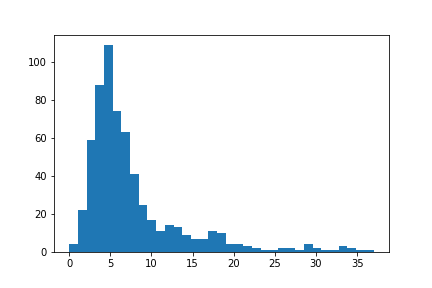
\includegraphics[width=.8\linewidth]{predictions_bin10_histogramm}
  \captionof{figure}{A figure}
  \label{fig:bsp_plot_good}
\end{minipage}%
\begin{minipage}{.5\textwidth}
  \centering
  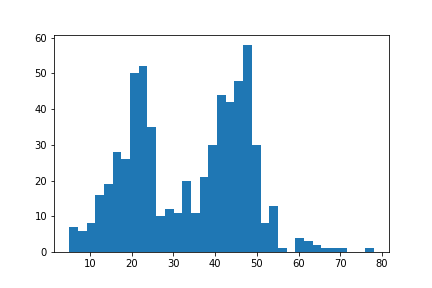
\includegraphics[width=.8\linewidth]{predictions_bin12_histogramm}
  \captionof{figure}{Another figure}
  \label{fig:bsp_plot_bad}
\end{minipage}
\end{figure}

\section{Experimente}

In diesem Abschnitt wird beschrieben welche Trainingsversuche durchgeführt wurden um ein bestmögliches Ergebnis zu erhalten. Die Beschreibungen für jeden Trainingsversuch sind jeweils in fünf Abschnitte unterteilt. Dazu gehört eine Einführung, das Datenset, eine Auflistung der veränderten Parameter, die Ergebnisse und ein Fazit.

Bevor die Beschreibung der jeweiligen Experimenten beginnt, hier eine Auflistung der Standard Parameter der Modelle. 

\begin{verbatim}
model.summary():
________________________________________________________________________________
Layer (type)                    Output Shape         Param #     Connected to

================================================================================
input_1 (InputLayer)            (None, 256, 256, 3)  0
________________________________________________________________________________
input_2 (InputLayer)            (None, 48, 20)       0
________________________________________________________________________________
sequential_1 (Sequential)       (None, 48, 1024)     104098080   input_1[0][0]
________________________________________________________________________________
sequential_2 (Sequential)       (None, 48, 128)      209920      input_2[0][0]
________________________________________________________________________________
concatenate_1 (Concatenate)     (None, 48, 1152)     0           sequential_1[1][0]
                                                                 sequential_2[1][0]
________________________________________________________________________________
lstm_3 (LSTM)                   (None, 48, 512)      3409920     concatenate_1[0][0]
________________________________________________________________________________
lstm_4 (LSTM)                   (None, 512)          2099200     lstm_3[0][0]
________________________________________________________________________________
dense_3 (Dense)                 (None, 20)           12312       lstm_4[0][0]
================================================================================
\end{verbatim}

Wichtig hierbei sind folgende drei Ebenen des Modells; \texttt{sequential\_1}, \texttt{sequential\_2} und \texttt{concatenate\_1}. 

\begin{description}
	\item[\texttt{sequential\_1}] Dieser Teil ist ein CNN, welches den Screenshot der Website als Input bekommen.
	\item[\texttt{sequential\_2}] Das Sprach Modell, ein rekurrentes Netzwerk, dass die DSL erlernt.
	\item[\texttt{concatenate\_1}] Hier wird der Output des CNN und des Sprach-Modells zusammen geführt und in ein weiteres rekurrentes Netzwerk gegeben welches aus der Sprache und dem Screenshot die Beschreibung dazu findet.
\end{description}

Weitere Hyper-Parameter:
\begin{description}
	\item[Anzahl Netzwerk Paramerter] Insgesamt hat das Netzwerk 109.829.432 trainierbare Parameter und kommt damit auf eine Größe von knapp 420 Mega Byte.
	\item[\texttt{CONTEXT\_LENGTH}] Die \texttt{CONTEXT\_LENGTH} auf 48 Tokens eingestellt. Die \texttt{CONTEXT\_LENGTH} bestimmt die Größe des Sliding-Windows, mit dem die Input Token Sequenzen abgearbeitet werden. 
	\item[\texttt{IMAGE\_SIZE}] Die Größe der Input Bilder ist 256 mal 256 Pixel.
	\item[\texttt{BATCH\_SIZE}] Trainiert wird in Batches mit jeweils 64 Bildern
	\item[\texttt{EPOCHS}] Es werden 10 Epochen trainiert.
	\item[\texttt{STEPS\_PER\_EPOCH}] In jeder Epoche weren 72.000 Schritte gemacht.
	
\end{description}

\subsection*{Training}

Da es für jeden Screenshot eine zugehörige Token-Sequenz mit variabler Länge gibt, müssen die Trainingsdaten mit einem Sliding-Window-Prinzip abgearbeitet werden. Dafür werden aus der Token-Sequenz, $n$ Samples gebildet, wobei $n = len(token\_sequence) - CONTEXT\_LENGTH$. Das Modell bekommt pro Screenshot $n$ Paare aus Screenshot und dazugehörigen Token-Kontext. Wichtig hierbei ist, dem Modell mitzuteilen wann eine Sequenz beginnt und wieder endet, dafür gibt es einen \texttt{start}-Token sowie einen \texttt{end}-Token. Diese werden je als pre- bzw. suffix an die Token-Sequenz angefügt bevor die $n$ Samples gebaut werden. 

So kann während dem Training mit Backpropagation ein klassischer Multi-Class-Loss optimiert werden.
\begin{equation}
L(I, X) =  -\sum_{t=1}^T x_{t+1} log(y_t)
\end{equation}

Hierbei ist $x_{t+1}$ der erwartete Token, und $y_t$ der berechnete. Das Modell ist in einer Gesamtheit ableitbar , dies bedeutet, der CNN-Teil kann zusammen mit den beiden LSTMs optimiert werden. Wie im Original Paper, wurde mit RMSProp-Algorithmus trainiert, mit einer Learning Rate von $0,0001$. Außerdem wurden die Gradienten um die Numerische Stabilität zu erhöhen, werden die Output Gradienten in das Intervall $[-1,1]$ getrimmt. Es wird eine Dropout-Regulation genutzt als eine Maßnahme gegen Overfitting. Im CNN nach den Max-Pooling Ebenen mit 25\% und nach den Fully-Connected Ebenen mit 30\%.



\subsection{1. Trainingsversuch}

\subsubsection*{Einführung}

Um eine Baseline aller weiteren Ergebnisse zu erstellen, wird das Original Modell aus dem pix2code Paper mit meinen neuen Daten neu trainiert. 

\subsubsection*{Datenset}

Das verwendete Datenset enthält 4128 Bilder, von denen 2890 für das Training verwendet werden. Die, das Datenset beschreibende, DSL enthält 24 Token. Jedes Bild wird mit durchschnittlich 62,47 Token (Median: 65) beschrieben, die maximale Anzahl liegt bei 92 Token, die minimale Anzahl bei 16. 

\subsubsection*{Veränderte Parameter}

Für diese Baseline wurden alle Parameter unverändert übernommen. Die einzige Anpassung die gemacht werden mussen, sind zwei Ebenen im Netzwerk, dessen Input und Output die Anzahl der Token reflektieren. Dies sind Ebene \texttt{input\_2} und \texttt{dense\_3}. Der Shape der beiden Ebenen wurde angepasst um mit 24 Token arbeiten zu können. Daher ist dieser in der Input-Ebene \texttt{(None, 48, 24)} anstatt \texttt{(None, 48, 20)}. Ebense bei der Dense-Ebene \texttt{(None, 24)} anstatt \texttt{(None, 20)}.

\subsubsection*{Ergebnis}

Nach dem Training des Netzwerkes, wurden mehrere zufällige Bilder ($n=10$) aus dem Test Set ausgewertet. Bei jedem einzelnen der Bilder kommt das selbe Ergebnis:

\begin{verbatim}
body {
	sidebar {
		sidebar-element,sidebar-element,sidebar-element,sidebar-element
	},
	row {
		quadruple {
			small-title,text,btn-inactive-blue
		},
		quadruple {
			small-title,text,btn-inactive-blue
		},
		double {
			small-title,text,btn-inactive-blue
		}
	},
	row {
		quadruple {
			small-title,text,btn-inactive-blue
		},
		quadruple {
			small-title,text,btn-inactive-blue
		},
		double {
			small-title,text,btn-inactive-blue
		}
	},
	row {
		quadruple {
			small-title,text,btn-inactive-blue
		},
		quadruple {
			small-title,text,btn-inactive-blue
		},
		double {
			small-title,text,btn-inactive-blue
		}
}
\end{verbatim}

\subsubsection*{Fazit}

Anhand des Ergebnisses kann man sagen, dass entweder die erhöhte Token Anzahl, oder die neuen Trainingsbilder, zu viel Entropie in die Trainingsdaten bringen. So kann das Modell leider zu keinem sinnvollen Optimum konvergieren. 


\subsection{2. Trainingsversuch}

\subsubsection*{Einführung}

In diesem Versuch wurde eine vergrößerte Context-Länge erprobt. Da im ersten Versuch, das Training nicht funktioniert hat, vermute ich den Fehler in einem zu kleinen Sichtbereich des LSTMs. Da durch die Token-Länge die Sichtbarkeit der Long-Term-Dependencies geregelt wird, verdoppel ich diese um zu sehen ob dadurch ein verbessertes Ergebnis zustande kommt.

\subsubsection*{Datenset}

Gleichbleibend zum ersten Versuch.

\subsubsection*{Veränderte Parameter}

Das Modell ist genau gleich wie im ersten Versuch, lediglich die Context-Länge wurde von 48 auf 96 erhöht.

\subsubsection*{Ergebnis}

Wie bei ersten Versuch ergibt dieses Training wieder der gleichen Output. Egal welches Bild als Input genommen wird. Um sicher zu gehen, dass diese Prediction nicht zufällig von dem gewählten Testbild abhängt, habe ich insgesamt 313 Bilder getestet, um festzustellen das alle diese Bilder zum gleichen Ergebnis führen. Alle dieser Bilder bekommen den exakt gleichen Output

\subsubsection*{Fazit}

An einem zu geringen Kontext kann das nicht konvergierende Training nicht liegen. In den folgenden Versuchen werden andere Parameter verändert.

\subsection{3. Trainingsversuch}


\subsubsection*{Einführung}

Da im ersten und zweiten Versuch, mit der Original Architektur kein brauchbares Ergebnis heraus gekommen ist, und das Netz ein zu falsches Ergebnis liefert, wird nun versucht mit einer höheren Komplexität der LSTMs ein Modell zu finden das besser funktioniert.

\subsubsection*{Datenset}

Gleichbleibend zum ersten Versuch.

\subsubsection*{Veränderte Parameter}

Hier hab ich die Anzahl der LSTM \texttt{units} von 128, im Language Modell, auf 192 erhöht. Außerdem erfolgte eine Veränderung der LSTM \texttt{units} von 512 auf 768 im Decoder Modell.

\begin{verbatim}
________________________________________________________________________________
Layer (type)                    Output Shape         Param #     Connected to
================================================================================
input_1 (InputLayer)            (None, 256, 256, 3)  0
________________________________________________________________________________
input_2 (InputLayer)            (None, 48, 24)       0
________________________________________________________________________________
sequential_3 (Sequential)       (None, 48, 1024)     104098080   input_1[0][0]
________________________________________________________________________________
sequential_4 (Sequential)       (None, 48, 192)      462336      input_2[0][0]
________________________________________________________________________________
concatenate_1 (Concatenate)     (None, 48, 1216)     0           sequential_3[1][0]
                                                                 sequential_4[1][0]
________________________________________________________________________________
lstm_3 (LSTM)                   (None, 48, 768)      6097920     concatenate_1[0][0]
________________________________________________________________________________
lstm_4 (LSTM)                   (None, 768)          4721664     lstm_3[0][0]
________________________________________________________________________________
dense_3 (Dense)                 (None, 24)           18456       lstm_4[0][0]
================================================================================
Total params: 115,398,456
Trainable params: 115,398,456
Non-trainable params: 0

________________________________________________________________________________
\end{verbatim}

Durch diese Veränderung gibt es ca. 8 Millionen mehr Parameter.
Die Länge des Kontextes wurde zurück auf 48 gestellt.

\subsubsection*{Ergebnis}

Exakt gleiches Ergebnis zu den beiden ersten Versuchen.

\subsubsection*{Fazit}

Da inzwischen immer noch der gleiche Output generiert wird, probiere ich nun einen Fehler im Programm-Code zu finden. Folgende Ursachen könnte es geben:

\begin{description}
	\item[Fehler im Sampler] Der Sampler generiert nach dem Training aus Screenshots die Token-Sequenz. Hier könnte zum einen, ein falsches Modell geladen werden, oder es wird fehlerhaft geladen.
	
	\begin{description}
		\item[Falsches Modell] Durch Umbenennung des Modells im Output Folder und Eingabe eines falschen Modellnamens, bricht das Programm jeweils ab.
		\item[Fehlerhaftes Laden] Die Ausgabe von \texttt{model.summary()} nach dem Laden des Modells ist identisch mit der erstellten während des Trainings.
	\end{description}
	
	\item[Fehler in den Daten] Während dem Preprocessing werden die Trainingsbilder in \texttt{numpy}-Arrays mit \texttt{shape(256,256,3} umgewandelt. Anschließend werden die Arrays und \texttt{gui}-Files zusammen abgespeichert.
	
	\begin{description}
		\item[Array Konvertierung] Beweis Bild + Nach optischer Kontrolle von zufälligen Samples ($n=10$) musste ich feststellen, dass diese korrekt sind.
		\item[Zuordnung Files] Nach Kontrolle zufälliger Samples sieht die Zuordnung ebenfalls gut aus.
	\end{description}
	
	\item[Fehler in Vocabulary] Es könnte auch an der fehlerhaften Abspeicherung der einzelnen Tokens liegen. Vocabulary und One-Hot-Encoding sind ebenfalls richtig.
	
	\item[Fehler im Datenset / -synthese] Hier wurde ein Fehler gefunden: Alle Screenshots, welche die \texttt{sidebar} anstatt des \texttt{menue} haben, sind doppelt enthalten. Der Grund hierfür, ist die Positionierung des Menü-Logos. Da es in Falle des \texttt{menue} zwei Möglichkeiten für die Positionierung des Logos gibt, wurden diese durch iteriert in der Erstellung der Daten. Da es bei der \texttt{sidebar} diese beiden Möglichkeiten aber nicht gab, wurden so alle Bilder mit der \texttt{sidebar} doppelt erstellt. Ein Viertel der Trainingsdaten hat ein Menü mit Logo links, ein weiteres Viertel hat das Logo rechts. Die andere Hälfte der Trainingsdaten hat die \texttt{sidebar}, in denen aber nur halb so viele einmalige enthalten sind.
	
\end{description}

\subsection{4. Trainingsversuch}


\subsubsection*{Einführung}

Nach dem Finden des Fehlers im vorherigen Versuch, wurde ein neues Datenset erstellt.

\subsubsection*{Datenset}

Ei neues Datenset mit 3096 Bildern wurde erstell. Ein Drittel hat das Feature \texttt{menue\_logo\_left}, ein Drittel \texttt{menue\_logo\_right}, und der Rest die \texttt{sidebar}. 

\subsubsection*{Veränderte Parameter}

In diesem Versuch wurden die gleichen Parameter wie im ersten Versuch genutzt.

\subsubsection*{Ergebnis}

Es erfolgte keine Verbesserung der Trainingsergebnisse. Die Token-Sequenz hat sich dahingehend geändert, dass nun anstatt der \texttt{sidebar} ein Menü in allen Ergebnissen ist.

\begin{verbatim}
body{
header{
logo-right,btn-inactive-white,btn-inactive-white
}
row{
quadruple{
small-titletextbtn-inactive-black
}
quadruple{
small-titletextbtn-inactive-black
}
double{
small-titletextbtn-inactive-black
}
}
row{
quadruple{
small-titletextbtn-inactive-black
}
quadruple{
small-titletextbtn-inactive-black
}
double{
small-titletextbtn-inactive-black
}
}
}
\end{verbatim}

\subsubsection*{Fazit}

Die gefundene Token Sequenz muss wohl die allgemeingültigste sein, da diese immer wieder gefunden wird. Da der Fehler nicht an einem Fehler im Programm liegt, muss er entweder in den Daten oder im Modell liegen. 

\subsection{5. Trainingsversuch}

\subsubsection*{Einführung}

Gleichzeitig zu dem 4. Versuch wurde noch ein Subset der Daten erstellt, das nur 70\% der Bilder aufweist. Dieses hat 2166 Bilder im Vergleich zu dem Set vom 4. Trainingsversuch. Der Gedanke hierbei ist, dass im Original Training vom pix2code Paper 1500 Trainingsbilder ausgereicht haben. Unter Umständen konvergiert es mit weniger Daten zu einem anderen Durchschnittswert oder fängt an die richtigen Ergebnisse herauszufinden.

\subsubsection*{Datenset}
Eine reduzierte Variante des Sets aus dem vierten Versuch.

\subsubsection*{Veränderte Parameter}

Gleiche Parameter wie im ersten Versuch.
bin8

\subsubsection*{Ergebnis}

Es erfolgte keine Verbesserung der Trainingsergebnisse.

\subsubsection*{Fazit}

Dieser Ansatz hat gezeigt, dass dieser Weg der falsche ist.

\subsection{6. Trainingsversuch}

\subsubsection*{Einführung}

Nach Analyse der Daten des Original Papers, wurde festgestellt, dass dort ein Tag weggelassen wurde. Es wird kein \texttt{body}-Tag verwendet. Dieser ist bei jedem der Bild-beschreibenden Token-Sequenzen der root-Knoten. Da er jedes mal auftritt, hat er aber keine Relevanz zu dem Screenshot und kann daher weggelassen werden.

\begin{verbatim}
python train.py ../../data/rfp_data_no_body_3096_11.10.
2018/train/ ../bin9/ 1

\end{verbatim}

\subsubsection*{Datenset}

Neues Datenset, ohne \texttt{body}-Tags. Dieses hat insgesamt 3096 Bilder und ist wieder 70-20-10 gesplittet in Trainings-, Test-, und Validierungsset. Durch das fehlen des \texttt{body}-Tags ergibt sich folgende Verteilungsmaße:
\begin{verbatim}
Token length analysis:
     mean token length:    59.69
     max token length:     89
     min token length:     14
     median token length:  62
\end{verbatim}

Die Median-Token-Länge ist um genau 3 Token geringer geworden. Dies liegt daran, dass zugehörig zum \texttt{body}-Tag zwei Klammern benötigt wurden (\texttt{\{} und \texttt{\}}), welche anzeigen dass der Rest der Token Kinds-Knoten des \texttt{body}-Tags sind.

\subsubsection*{Veränderte Parameter}

Gleiche Parameter wie im ersten Versuch.

\subsubsection*{Ergebnis}

Es kommt die gleiche Ergebnis-Sequenz wie bei den Versuchen davor heraus.

\begin{verbatim}

header{
logo-right,btn-inactive-white,btn-inactive-white
}
row{
quadruple{
small-title,text,btn-inactive-black
}
quadruple{
small-title,text,btn-inactive-black
}
double{
small-title,text,btn-inactive-black
}
}
row{
quadruple{
small-title,text,btn-inactive-black
}
quadruple{
small-title,text,btn-inactive-black
}
double{
small-title,text,btn-inactive-black
}
}

\end{verbatim}

Diesmal jedoch ohne \texttt{body}-Tag.


\subsubsection*{Fazit}

Das Scheitern des Trainings wurde nicht durch die Verkleinerung der DSL behoben. Als nächster Schritt sollte jeweils der Sprach- sowie das Bild-Teil des Modells näher in Betracht genommen werden. Ein Großteil der Parameter des Modells sind bereits im CNN (hier erfolgt die Analyse des Bildes), deswegen wird es die Gesamtperformance weniger stark verbessern wenn man die gleiche Zahl an neuen Parametern hier hinzufügt. Deswegen wird zunächst der Sprach- und der Decoder-Teil des Modell untersucht.

\subsection{7. Trainingsversuch}

%Versuch mit GRUs \cite{GRUvsLSTM} \cite{lstmSearchSpace}
%bin10

\subsubsection*{Einführung}

Wie im Fazit des vorangegangen Versuchs, wird nun daran gearbeit, die LSTMs, welche der sprach analysierende und der decodierende Teil des Modells sind zu verbessern. Nach der Lektüre eines Posts von Colahs Blog, wurden testweise die klassischen LSTMs durch GRUs ersetzt.

\subsubsection*{Datenset}

Hier wurde das Datenset aus dem sechsten Trainingsversuch verwendet.

\subsubsection*{Veränderte Parameter}

\begin{verbatim}
________________________________________________________________________________
Layer (type)                    Output Shape         Param #     Connected to
================================================================================
input_1 (InputLayer)            (None, 256, 256, 3)  0
________________________________________________________________________________
input_2 (InputLayer)            (None, 48, 23)       0
________________________________________________________________________________
sequential_1 (Sequential)       (None, 48, 1024)     104098080   input_1[0][0]
________________________________________________________________________________
sequential_2 (Sequential)       (None, 48, 128)      157056      input_2[0][0]
________________________________________________________________________________
concatenate_1 (Concatenate)     (None, 48, 1152)     0           sequential_1[1][0]
                                                                 sequential_2[1][0]
________________________________________________________________________________
gru_3 (GRU)                     (None, 48, 512)      2557440     concatenate_1[0][0]
________________________________________________________________________________
gru_4 (GRU)                     (None, 512)          1574400     gru_3[0][0]
________________________________________________________________________________
dense_3 (Dense)                 (None, 23)           11799       gru_4[0][0]
================================================================================

Trainable params: 108,398,775

\end{verbatim}

Die LSTMs in \texttt{sequential\_2} sowie in Ebene 3 und 4 wurden durch GRUs ersetzt. Die Anzahl der \texttt{units} wurde beibehalten (128 bzw. 512). Dadurch, dass im GRU die Input- und Forget-Gates gekoppelt sind, hat das Modell jetzt eine Millionen Parameter weniger.

\subsubsection*{Ergebnis}

Anstatt der bereits mehrmals auftretenden Token Abfolge, gelingt es diesem Modell richtige Predictions zu erstellten. Alle der 619 getesteten Files konnten ohne Fehler compiliert werden. Die Analyse der Fehlerverteilung ergibt folgende Lageparameter in Abbildung~\ref{fig:lage_bin10}. Die Verteilung der Fehleranzahlen ist in Abbildung~\ref{fig:hist_bin10} gegeben.



\begin{figure}
\centering
\begin{minipage}{.5\textwidth}
  \centering
  \begin{description}
	\item[Arithmetisches Mittel] $7.82$	
	\item[Geometrisches Mittel] $6.36$
	\item[Harmonisches Mittel] $5.34$
	\item[Quintile] p20: $4$, p40: $5$, p60: $7$, p80: $10$
	\item[Median] $6$
	\item[Modus] $5$
	\item[Vorkommen Modus] $109$
	\item[Gesamt Fehler Score] 4840
	\item[Anzahl Token Testset] 36751 
	\item[Anzahl generierter Token] 36186
	\item[Score pro Token in Testset] 0.1317
\end{description}
  \captionof{figure}{Lageparameter}
  \label{fig:lage_bin10}
\end{minipage}%
\begin{minipage}{.5\textwidth}
  \centering
  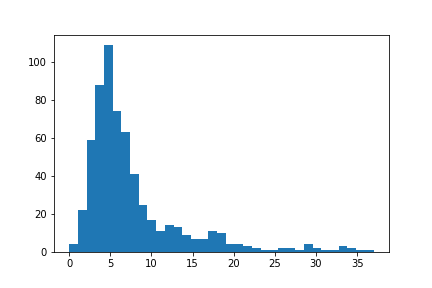
\includegraphics[width=1\linewidth]{predictions_bin10_histogramm}
  \captionof{figure}{Fehlerverteilung}
  \label{fig:hist_bin10}
\end{minipage}
\end{figure}



\begin{comment}
\begin{figure}
\centering
\begin{minipage}{.5\textwidth}
  \centering
  \begin{description}
	\item[Arithmetisches Mittel] $13.98$	
	\item[Geometrisches Mittel] $11.33$
	\item[Harmonisches Mittel] $8.73$
	\item[Quintile] p20: $6$, p40: $9$, p60: $16$, p80: $23$
	\item[Median] $12$
	\item[Modus] $7$
	\item[Vorkommen Modus] $46$
	\item[Gesamt Fehler Score]
	\item[Anzahl generierter Token]
	\item[Score pro Token]
\end{description}
  \captionof{figure}{Lageparameter}
  \label{fig:lage_bin12}
\end{minipage}%
\begin{minipage}{.5\textwidth}
  \centering
  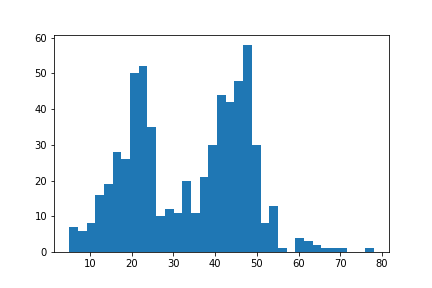
\includegraphics[width=1\linewidth]{predictions_bin12_histogramm}
  \captionof{figure}{Fehlerverteilung}
  \label{fig:hist_bin12}
\end{minipage}
\end{figure}
\end{comment}

Im weiteren wird das letzte Quintil der Fehler analysiert und mit dem Rest verglichen. In der Abbildung~\ref{fig:fehler_gesamt_bin10} ist die Fehlerverteilung aller Testdaten zusehen, in Abbildung~\ref{fig:fehler_beste80_bin10} die besten 80\% und in Abbildung~\ref{fig:fehler_schlechteste20_bin10} die schlechtesten 20\%. 

\begin{figure}
\centering
\begin{minipage}{.33\textwidth}
  \centering
  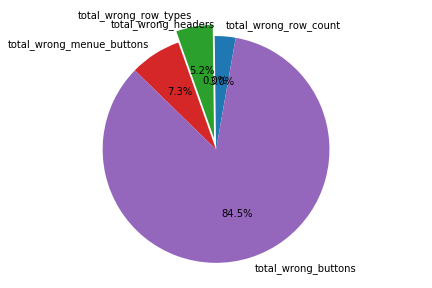
\includegraphics[width=1\linewidth]{predictions_bin10_total_error_types_pie_chart}
  \captionof{figure}{Gesamt}
  \label{fig:fehler_gesamt_bin10}
\end{minipage}%
\begin{minipage}{.33\textwidth}
  \centering
  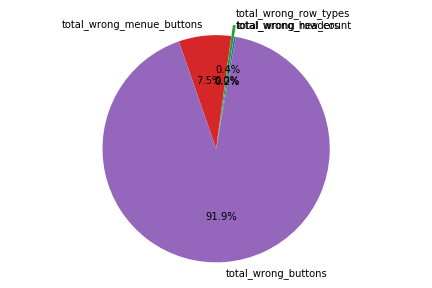
\includegraphics[width=1\linewidth]{predictions_bin10_excluded_p80_error_types_pie_chart}
  \captionof{figure}{Ohne p80}
  \label{fig:fehler_beste80_bin10}
\end{minipage}
\begin{minipage}{.33\textwidth}
  \centering
   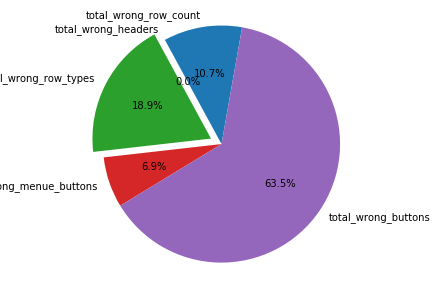
\includegraphics[width=1\linewidth]{predictions_bin10_p80_error_types_pie_chart}
  \captionof{figure}{Nur p80}
  \label{fig:fehler_schlechteste20_bin10}
\end{minipage}%
\end{figure}

Bei 80\% aller Testdaten sind die Fehleruhrsachen zu 92\% ausschließlich falsche Buttons! Außerdem ist die Verteilung der Row Types über den Testdaten sehr genau, wie in Abbildung~\ref{fig:bin10_row_type} zu sehen ist. Mit einer Perfekten Prediction müsste jeder Row Type mit $16,\frac{2}{3}\%$ vorliegen.

\begin{figure}[h]
\centering
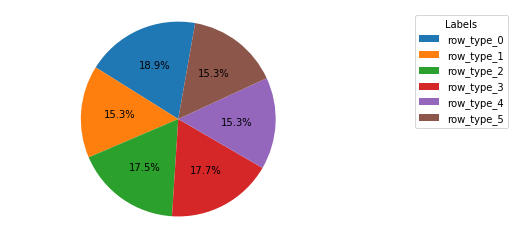
\includegraphics[width=0.3\textwidth]{predictions_bin10_predicted_row_type_distribution}
\caption{Verteilung Row Types}
\label{fig:bin10_row_type}
\end{figure}


\subsubsection*{Fazit}

Dieses Training war ein voller Erfolg. Es ergibt eine hohe Testgenauigkeit und es hat weniger Parameter als das Original Modell aus dem Paper. 

\begin{comment}
4010/4009 [==============================] - 1565s 390ms/step - loss: 0.3897
Epoch 2/10
4010/4009 [==============================] - 1555s 388ms/step - loss: 0.1842
Epoch 3/10
4010/4009 [==============================] - 1555s 388ms/step - loss: 0.1669
Epoch 4/10
4010/4009 [==============================] - 1546s 386ms/step - loss: 0.1543
Epoch 5/10
4010/4009 [==============================] - 1528s 381ms/step - loss: 0.1442
Epoch 6/10
4010/4009 [==============================] - 1528s 381ms/step - loss: 0.1331
Epoch 7/10
4010/4009 [==============================] - 1528s 381ms/step - loss: 0.1240
Epoch 8/10
4010/4009 [==============================] - 1530s 381ms/step - loss: 0.1191
Epoch 9/10
4010/4009 [==============================] - 1529s 381ms/step - loss: 0.1157
Epoch 10/10
4010/4009 [==============================] - 1528s 381ms/step - loss: 0.1135
\end{comment}

\subsection{8. Trainingsversuch}

%language modell: LSTM
%Decoder: GRU
%bin11


\subsubsection*{Einführung}

In diesem Versuch wird eine Kombination aus der Original Architektur mit LSTMs und der neuen mit GRUs aus dem siebten Trainingsversuch getestet. Das Sprach-Modell wird wie im Original mit LSTMs gebildet, der Decoder hingegen mit den GRUs. 

\subsubsection*{Datenset}

Hier wurde das Datenset aus dem sechsten Trainingsversuch verwendet.

\subsubsection*{Veränderte Parameter}

Wie folgt wurde das Modell verändert:
\begin{verbatim}

Layer (type)                    Output Shape         Param #     Connected to
================================================================================
input_1 (InputLayer)            (None, 256, 256, 3)  0
________________________________________________________________________________
input_2 (InputLayer)            (None, 48, 23)       0
________________________________________________________________________________
sequential_1 (Sequential)       (None, 48, 1024)     104098080   input_1[0][0]
________________________________________________________________________________
sequential_2 (Sequential)       (None, 48, 128)      209408      input_2[0][0]
________________________________________________________________________________
concatenate_1 (Concatenate)     (None, 48, 1152)     0           sequential_1[1][0]
                                                                 sequential_2[1][0]
________________________________________________________________________________
gru_1 (GRU)                     (None, 48, 512)      2557440     concatenate_1[0][0]
________________________________________________________________________________
gru_2 (GRU)                     (None, 512)          1574400     gru_1[0][0]
________________________________________________________________________________
dense_3 (Dense)                 (None, 23)           11799       gru_2[0][0]
================================================================================

Trainable params: 108,451,127

\end{verbatim}

Die Ebene \texttt{sequential\_2} ist durch ein LSTM realisiert, die Ebenen \texttt{gru\_1} und \texttt{gru\_2} jeweils durch ein GRU. 

\subsubsection*{Ergebnis}

Jeder der getesteten Daten erzeugt den selben Output:
\begin{verbatim}
header{
logo-right,btn-inactive-white,btn-inactive-white
}
row{
quadruple{
small-title,text,btn-inactive-black
}
quadruple{
small-title,text,btn-inactive-black
}
double{
small-title,text,btn-inactive-black
}
}
row{
quadruple{
small-title,text,btn-inactive-black
}
quadruple{
small-title,text,btn-inactive-black
}
double{
small-title,text,btn-inactive-black
}
}
\end{verbatim}

\subsubsection*{Fazit}

Dieses Ergebnis legt Nahe, dass das Bottleneck des Modells in dem Sprach-Modell liegt. 

\subsection{9. Trainingsversuch}


%language modell: GRU
%Decoder: LSTM
\begin{comment}
python train.py ../../data/rfp_data_no_body_3096_11.10.
2018/train/ ../bin12/ 1

4010/4009 [==============================] - 1646s 410ms/step - loss: 0.5490
Epoch 2/10
4010/4009 [==============================] - 1643s 410ms/step - loss: 0.1962
Epoch 3/10
4010/4009 [==============================] - 1642s 410ms/step - loss: 0.1932
Epoch 4/10
4010/4009 [==============================] - 1642s 410ms/step - loss: 0.1920
Epoch 5/10
4010/4009 [==============================] - 1632s 407ms/step - loss: 0.1916
Epoch 6/10
4010/4009 [==============================] - 1615s 403ms/step - loss: 0.1917
Epoch 7/10
4010/4009 [==============================] - 1616s 403ms/step - loss: 0.1940
Epoch 8/10
4010/4009 [==============================] - 1616s 403ms/step - loss: 0.1869
Epoch 9/10
4010/4009 [==============================] - 1616s 403ms/step - loss: 0.1854
Epoch 10/10
4010/4009 [==============================] - 1609s 401ms/step - loss: 0.1783
\end{comment}


\subsubsection*{Einführung}

Nach dem Testen ob es reicht allein den Decoder durch ein GRU zu ersetzten reicht um das Modell konvergieren zu lassen, wird nun getestet, ob es ausreicht das Sprach-Modell mit dem GRU zu realisieren.

\subsubsection*{Datenset}

Hier wurde das Datenset aus dem sechsten Trainingsversuch verwendet.

\subsubsection*{Veränderte Parameter}

Wie bereits in dem Original Paper, ist hier der Decoder mit LSTMs realisiert, zusehen in den Ebenen \texttt{lstm\_1} und \texttt{lstm\_1}. Die Ebene \texttt{sequential\_2} ist wie im erfolgreichen siebten Trainingsversuch ein GRU.

\begin{verbatim}
Layer (type)                    Output Shape         Param #     Connected to
===============================================================================
input_1 (InputLayer)            (None, 256, 256, 3)  0
_______________________________________________________________________________
input_2 (InputLayer)            (None, 48, 23)       0
_______________________________________________________________________________
sequential_1 (Sequential)       (None, 48, 1024)     104098080   input_1[0][0]
_______________________________________________________________________________
sequential_2 (Sequential)       (None, 48, 128)      157056      input_2[0][0]
_______________________________________________________________________________
concatenate_1 (Concatenate)     (None, 48, 1152)     0           sequential_1[1][0]
                                                                 sequential_2[1][0]
_______________________________________________________________________________
lstm_1 (LSTM)                   (None, 48, 512)      3409920     concatenate_1[0][0]
_______________________________________________________________________________
lstm_2 (LSTM)                   (None, 512)          2099200     lstm_1[0][0]
_______________________________________________________________________________
dense_3 (Dense)                 (None, 23)           11799       lstm_2[0][0]
===============================================================================

Trainable params: 109,776,055

\end{verbatim}

Durch das Benutzen von LSTMs im Decoder, ist die Anzahl der Parameter wieder auf knappe 110 Millionen gewachsen.

\subsubsection*{Ergebnis}

Ähnlich wie das siebte Training konnte das Netzwerk konvergieren und einen nicht allgemeinen Output erzeugen. Die Analyse der Testdaten zeigte jedoch, dass insgesamt 143 der 619 Daten nicht kompiliert werden konnten. 

Die Analyse der Fehlerverteilung ergibt folgende Lageparameter in Abbildung~\ref{fig:lage_bin12}. Die Verteilung der Fehler-Scores ist in Abbildung~\ref{fig:hist_bin12} gegeben.

\begin{figure}
\centering
\begin{minipage}{.5\textwidth}
  \centering
  \begin{description}
	\item[Arithmetisches Mittel] $33.50$	
	\item[Geometrisches Mittel] $30.23$
	\item[Harmonisches Mittel] $26.45$
	\item[Quintile] p20: $20$, p40: $26$, p60: $41$, p80: $46$
	\item[Median] $36$
	\item[Modus] $46$
	\item[Vorkommen Modus] $32$
	\item[Gesamt Fehler Score] 20734
	\item[Anzahl Token Testset] 36751 
	\item[Anzahl generierter Token] 49012
	\item[Score pro Token in Testset] 0.56
\end{description}
  \captionof{figure}{Lageparameter}
  \label{fig:lage_bin12}
\end{minipage}%
\begin{minipage}{.5\textwidth}
  \centering
  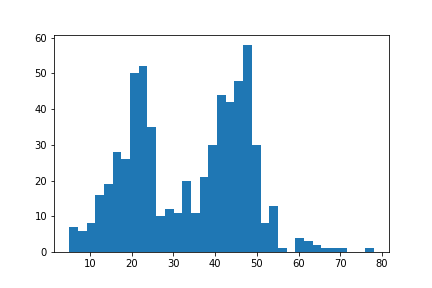
\includegraphics[width=1\linewidth]{predictions_bin12_histogramm}
  \captionof{figure}{Fehlerverteilung}
  \label{fig:hist_bin12}
\end{minipage}
\end{figure}

Der Vergleich zu den Lageparametern~\ref{fig:lage_bin10} des siebten Experiment, performt dieses Modell sehr viel schlechter. Die Median Fehler-Score dieses Experiments ist fünfmal so hoch wie die des siebtens.

Im weiteren wird das letzte Quintil der Fehler analysiert und mit dem Rest verglichen. In der Abbildung~\ref{fig:fehler_gesamt_bin12} ist die Fehlerverteilung aller Testdaten zusehen, in Abbildung~\ref{fig:fehler_beste80_bin12} die besten 80\% und in Abbildung~\ref{fig:fehler_schlechteste20_bin12} die schlechtesten 20\%. 

\begin{figure}
\centering
\begin{minipage}{.33\textwidth}
  \centering
  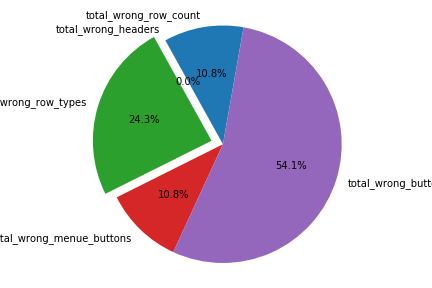
\includegraphics[width=1\linewidth]{predictions_bin12_total_error_types_pie_chart}
  \captionof{figure}{Gesamt}
  \label{fig:fehler_gesamt_bin12}
\end{minipage}%
\begin{minipage}{.33\textwidth}
  \centering
  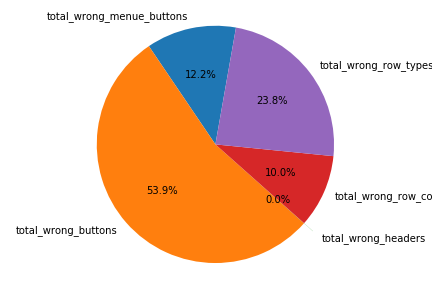
\includegraphics[width=1\linewidth]{predictions_bin12_excluded_p80_error_types_pie_chart}
  \captionof{figure}{Ohne p80}
  \label{fig:fehler_beste80_bin12}
\end{minipage}
\begin{minipage}{.33\textwidth}
  \centering
   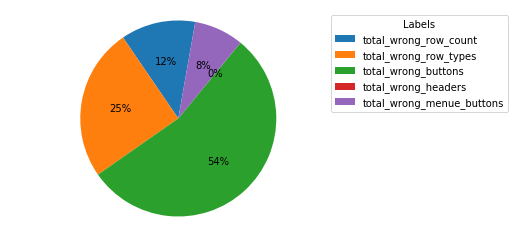
\includegraphics[width=1\linewidth]{predictions_bin12_p80_error_types_pie_chart}
  \captionof{figure}{Nur p80}
  \label{fig:fehler_schlechteste20_bin12}
\end{minipage}%
\end{figure}

Der Unterschied in der Verteilung der Fehlertypen zwischen den ersten 4 Quintilen und dem letzten Quintil ist hier viel geringer als in dem siebten Experiment. Diesem Modell ist es nicht gelungen, gute Ergebnisse aus den Trainingsdaten zu generieren. Dies unterstreicht die Verteilung der generierten Row Types in Abbildung~\ref{fig:bin12_row_type}. Hier ist zusehen, dass das Modell es nicht lernen konnten die verschiedenen Typen sicher zu unterscheiden. Ein Großteil wird als Typ 4 erkannt, ca. 60\%, und der Rest ist nicht regelmäßig verteilt.

\begin{figure}[h]
\centering
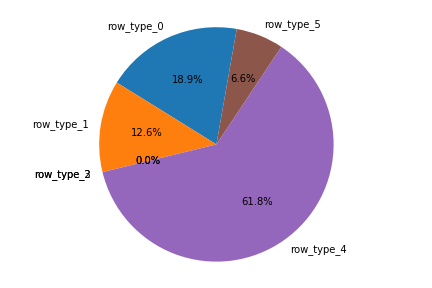
\includegraphics[width=0.3\textwidth]{predictions_bin12_predicted_row_type_distribution}
\caption{Verteilung Row Types}
\label{fig:bin12_row_type}
\end{figure}

\subsubsection*{Fazit}





\subsection{10. Trainingsversuch}

\begin{comment}
%Language: LSTM 256 units
%Decoder 512 units

python train.py ../../data/rfp_data_no_body_3096_11.10.
2018/ ../bin13/ 1

4010/4009 [==============================] - 1737s 433ms/step - loss: 0.7700
Epoch 2/10
4010/4009 [==============================] - 1730s 431ms/step - loss: 0.2034
Epoch 3/10
4010/4009 [==============================] - 1755s 438ms/step - loss: 0.1963
Epoch 4/10
4010/4009 [==============================] - 1742s 434ms/step - loss: 0.1945
Epoch 5/10
4010/4009 [==============================] - 1725s 430ms/step - loss: 0.1929
Epoch 6/10
4010/4009 [==============================] - 1726s 430ms/step - loss: 0.1923
Epoch 7/10
4010/4009 [==============================] - 1725s 430ms/step - loss: 0.1931
Epoch 8/10
4010/4009 [==============================] - 1724s 430ms/step - loss: 0.1923
Epoch 9/10
4010/4009 [==============================] - 1725s 430ms/step - loss: 0.1924
Epoch 10/10
4010/4009 [==============================] - 1725s 430ms/step - loss: 0.1920
\end{comment}



\subsubsection*{Einführung}

Mit diesem Versuch, wird getestet, ob eine reine LSTM-Lösung mit mehr Parametern funktionieren könnte. 

\subsubsection*{Datenset}

Hier wurde das Datenset aus dem sechsten Trainingsversuch verwendet.

\subsubsection*{Veränderte Parameter}

Um zu überprüfen, ob es reicht das Sprach-Modell komplexer zu gestalten, wurde die Anzahl der LSTM Units dieses Teils verdoppelt. 

\begin{verbatim}

Layer (type)                    Output Shape         Param #     Connected to
==============================================================================
input_1 (InputLayer)            (None, 256, 256, 3)  0
______________________________________________________________________________
input_2 (InputLayer)            (None, 48, 23)       0
______________________________________________________________________________
sequential_1 (Sequential)       (None, 48, 1024)     104098080   input_1[0][0]
______________________________________________________________________________
sequential_2 (Sequential)       (None, 48, 256)      812032      input_2[0][0]
______________________________________________________________________________
concatenate_1 (Concatenate)     (None, 48, 1280)     0           sequential_1[1][0]
                                                                 sequential_2[1][0]
______________________________________________________________________________
lstm_3 (LSTM)                   (None, 48, 512)      3672064     concatenate_1[0][0]
______________________________________________________________________________
lstm_4 (LSTM)                   (None, 512)          2099200     lstm_3[0][0]
______________________________________________________________________________
dense_3 (Dense)                 (None, 23)           11799       lstm_4[0][0]
==============================================================================

Total params: 110,693,175
\end{verbatim}

In der Ebene \texttt{sequential\_2}, kommen 256 anstatt 128 Units vor.

\subsubsection*{Ergebnis}

Das Training konvergierte, erzeugt ein sehr schlechtes Ergebnis. Es konnten zwar alle 619 Testdaten kompiliert werden, die Scorings sind aber nicht Konkurrenzfähig zu den siebten Versuch - aber besser als die Ergebnisse des Neuntens.

Die Analyse der Fehlerverteilung ergibt folgende Lageparameter in Abbildung~\ref{fig:lage_bin13}. Die Verteilung der Fehler-Scores ist in Abbildung~\ref{fig:hist_bin13} gegeben.

\begin{figure}
\centering
\begin{minipage}{.5\textwidth}
  \centering
  \begin{description}
	\item[Arithmetisches Mittel] $23.81$	
	\item[Geometrisches Mittel] $22.98$
	\item[Harmonisches Mittel] $22.14$
	\item[Quintile] p20: $19$, p40: $22$, p60: $24$, p80: $31$
	\item[Median] $23$
	\item[Modus] $22$
	\item[Vorkommen Modus] $57$
	\item[Gesamt Fehler Score] 14739
	\item[Anzahl Token Testset] 36751 
	\item[Anzahl generierter Token] 34664
	\item[Score pro Token Testset]  0.40
\end{description}
  \captionof{figure}{Lageparameter}
  \label{fig:lage_bin13}
\end{minipage}%
\begin{minipage}{.5\textwidth}
  \centering
  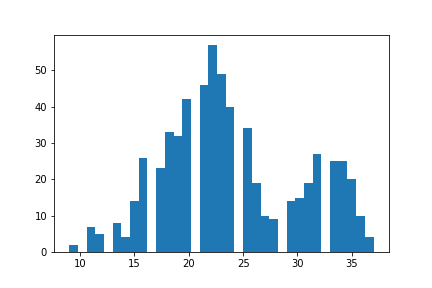
\includegraphics[width=1\linewidth]{predictions_bin13_histogramm}
  \captionof{figure}{Fehlerverteilung}
  \label{fig:hist_bin13}
\end{minipage}
\end{figure}

Auffallend ist hier, dass die Verteilung der Fehler Scores viel gleichmäßiger als in den Versuchen Sieben und Neun ist. Die Abstände der Verschiedenen Mittel sowie die der Quintile sind geringer. Im Vergleich zum neunten Versuch ist der Median Score um 10 geringer. 

\begin{figure}
\centering
\begin{minipage}{.33\textwidth}
  \centering
  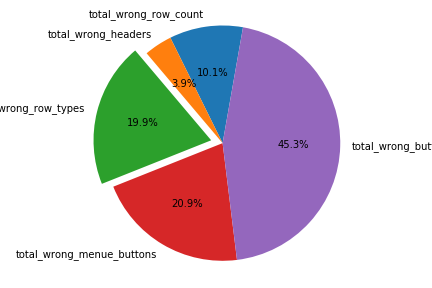
\includegraphics[width=1\linewidth]{predictions_bin13_total_error_types_pie_chart}
  \captionof{figure}{Gesamt}
  \label{fig:fehler_gesamt_bin13}
\end{minipage}%
\begin{minipage}{.33\textwidth}
  \centering
  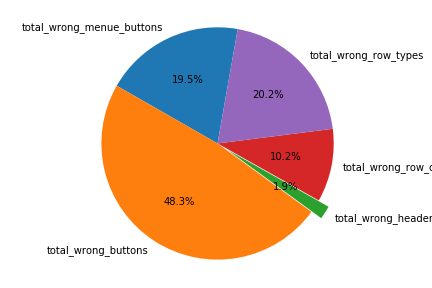
\includegraphics[width=1\linewidth]{predictions_bin13_excluded_p80_error_types_pie_chart}
  \captionof{figure}{Ohne p80}
  \label{fig:fehler_beste80_bin13}
\end{minipage}
\begin{minipage}{.33\textwidth}
  \centering
   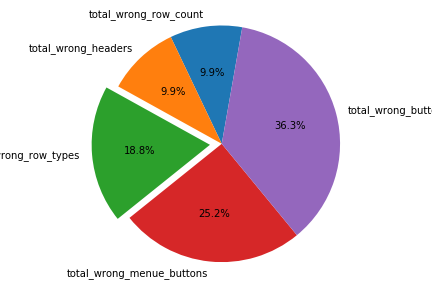
\includegraphics[width=1\linewidth]{predictions_bin13_p80_error_types_pie_chart}
  \captionof{figure}{Nur p80}
  \label{fig:fehler_schlechteste20_bin13}
\end{minipage}%
\end{figure}

Auffallend ist jedoch in Abbildung~\ref{fig:fehler_gesamt_bin13}, dass dieses Modell den bisher höchsten Anteil an falsch zugeordneten \texttt{header}-Elementen hat. Die bisherigen konvergierten Modelle konnten diese jeweils perfekt zuordnen. 

Schließlich kommt der letzte Punkt der Analyse, die Verteilung der generierten Row Typen. Hier schneidet dieses Modell am aller schlechtesten ab. Es generiert in für Datei aus dem Testset immer nur einen von zwei Row Types. 

\begin{figure}[h]
\centering
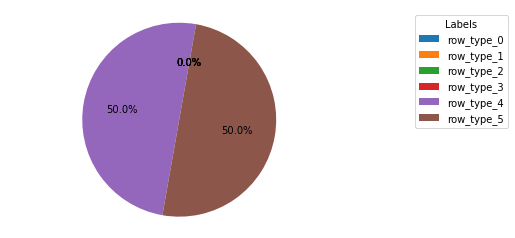
\includegraphics[width=0.3\textwidth]{predictions_bin13_predicted_row_type_distribution}
\caption{Verteilung Row Types}
\label{fig:bin13_row_type}
\end{figure}


\subsubsection*{Fazit}

Obwohl dieses Modell mit großer LSTM Architektur knappe 2.5 Millionen Parameter mehr hat, sind die Ergebnisse viel schlechter. Besonders die drei fehlenden Row Types fallen hier ins Gewicht. Zunächst wurde angenommen, dass dieses Modell gleich gut oder besser wie die reine GRU Architektur aus Versuch Sieben sein könnte. Die LSTMs performen bisher schlechter für diesen Task. 




\subsection{11. Trainingsversuch}
%Language: GRU 192 units
%Decoder GRU 768 units

%bin14

\subsubsection*{Einführung}
In diesem Versuch soll heraus gefunden werden, ob eine größere GRU-Architektur ein noch besseres Ergebniss liefern könnte.

\subsubsection*{Datenset}

Hier wurde das Datenset aus dem sechsten Trainingsversuch verwendet.


\subsubsection*{Veränderte Parameter}

Es wurden sowohl die Sprach-Ebene, als auch die Decoder-Ebene vergrößert.

\begin{verbatim}
Layer (type)                    Output Shape         Param #     Connected to
=============================================================================
input_1 (InputLayer)            (None, 256, 256, 3)  0
_____________________________________________________________________________
input_2 (InputLayer)            (None, 48, 23)       0
_____________________________________________________________________________
sequential_1 (Sequential)       (None, 48, 1024)     104098080   input_1[0][0]
_____________________________________________________________________________
sequential_2 (Sequential)       (None, 48, 192)      346176      input_2[0][0]
_____________________________________________________________________________
concatenate_1 (Concatenate)     (None, 48, 1216)     0           sequential_1[1][0]
                                                                 sequential_2[1][0]
_____________________________________________________________________________
gru_3 (GRU)                     (None, 48, 768)      4573440     concatenate_1[0][0]
_____________________________________________________________________________
gru_4 (GRU)                     (None, 768)          3541248     gru_3[0][0]
_____________________________________________________________________________
dense_3 (Dense)                 (None, 23)           17687       gru_4[0][0]
=============================================================================

Total params: 112,576,631

\end{verbatim}

Hier kann man sehen, dass in der Ebene \texttt{sequential\_2} in der Ebene \texttt{gru\_3} die Unit-Anzahl vergrößert wurde. Von 128 auf 192, bzw. von 512 auf 786.

\subsubsection*{Ergebnis}

Auch dieses Netz konvergiert, leider ist das Ergebnis gegenüber Versuch Sieben nicht besser geworden.

\begin{figure}
\centering
\begin{minipage}{.5\textwidth}
  \centering
  \begin{description}
	\item[Arithmetisches Mittel] $20.10$	
	\item[Geometrisches Mittel] $19.23$
	\item[Harmonisches Mittel] $18.38$
	\item[Quintile] p20: $16$, p40: $19$, p60: $21$, p80: $22$
	\item[Median] $20$
	\item[Modus] $21$
	\item[Vorkommen Modus] $85$
	\item[Gesamt Fehler Score] 12442
	\item[Anzahl Token Testset] 36751 
	\item[Anzahl generierter Token] 33680
	\item[Score pro Token Testset]  0.34
\end{description}
  \captionof{figure}{Lageparameter}
  \label{fig:lage_bin14}
\end{minipage}%
\begin{minipage}{.5\textwidth}
  \centering
  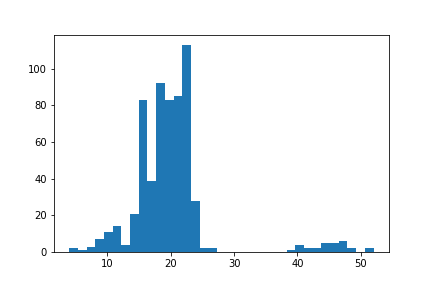
\includegraphics[width=1\linewidth]{predictions_bin14_histogramm}
  \captionof{figure}{Fehlerverteilung}
  \label{fig:hist_bin14}
\end{minipage}
\end{figure}

Der Hauptteil der Fehler-Scores liegt um die Zwanzig, mit ein paar wenigen im niedrigeren oder höheren Bereich. Zu sehen ist das sehr gut in der Abbildung~\ref{fig:hist_bin14}. 

\begin{figure}
\centering
\begin{minipage}{.33\textwidth}
  \centering
  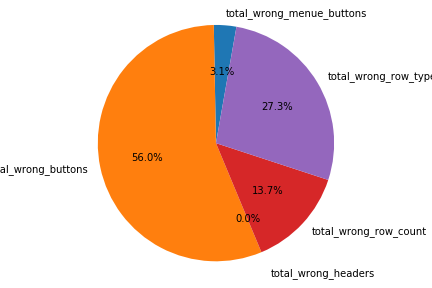
\includegraphics[width=1\linewidth]{predictions_bin14_total_error_types_pie_chart}
  \captionof{figure}{Gesamt}
  \label{fig:fehler_gesamt_bin14}
\end{minipage}%
\begin{minipage}{.33\textwidth}
  \centering
  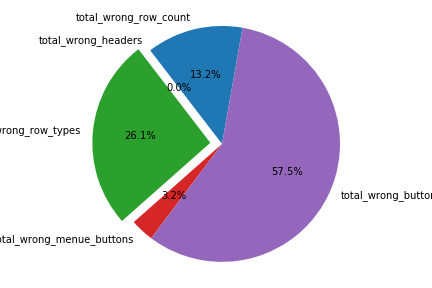
\includegraphics[width=1\linewidth]{predictions_bin14_excluded_p80_error_types_pie_chart}
  \captionof{figure}{Ohne p80}
  \label{fig:fehler_beste80_bin14}
\end{minipage}
\begin{minipage}{.33\textwidth}
  \centering
   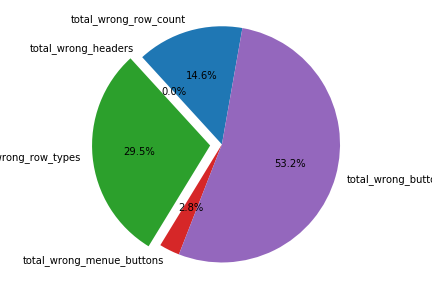
\includegraphics[width=1\linewidth]{predictions_bin14_p80_error_types_pie_chart}
  \captionof{figure}{Nur p80}
  \label{fig:fehler_schlechteste20_bin14}
\end{minipage}
\end{figure}

In Abbildungen ~\ref{fig:fehler_gesamt_bin14}-~\ref{fig:fehler_schlechteste20_bin14} ist zu sehen, dass die Verteilung der Fehler-Type nach Fehler Anzahl relativ gleichmäßig liegt. Die Daten, welche die Meisten Fehler erzeugt haben, erzeugen die gleichen Arten wie der Gesamtmenge. Daher liegt die Fehlerursache nicht in besonders komplexen Screenshots sondern bei einer schlechten Klassifizierung.

Schlussendlich ist zu sehen, wie schlecht das Modell bei der richtigen Einordnung von den Row Types anschneidet in Abbildung~\ref{fig:bin14_row_type}. Es kann nicht zwischen den einzelnen Typen unterscheiden.


\begin{figure}[h]
\centering
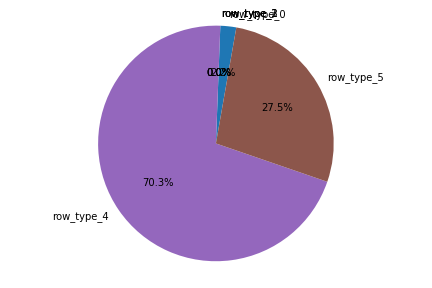
\includegraphics[width=0.3\textwidth]{predictions_bin14_predicted_row_type_distribution}
\caption{Verteilung Row Types}
\label{fig:bin14_row_type}
\end{figure}


\subsubsection*{Fazit}

Wieso performt dieses Modell, obwohl es doch größer ist so viel schlechter als Versuch Sieben? Hier hat man es mit einem klassischen Fall des Overfittings zu tun. Das Modell war hier so komplex, dass es die Beschreibungen aller Trainingsdaten auswendig lernen konnte. Dadurch sah das Training gut aus, das Testen hingegen zeigt, dass es nicht gut verallgemeinern konnte.


\subsection{12. Trainingsversuch}
%Language: GRU 128 units
%Decoder GRU 512 units
%CONTEXT_64
%bin15
\subsubsection*{Einführung}

In diesem Versuch wird überprüft, ob eine Vergrößerung der \texttt{CONTEXT\_LENGTH} das Ergebnis positiv beeinflusst, und wenn ja wie stark. 

\subsubsection*{Datenset}

Hier wurde das Datenset aus dem sechsten Trainingsversuch verwendet.

\subsubsection*{Veränderte Parameter}

Die \texttt{CONTEXT\_LENGTH} wurde von 48 auf 64 (Anmerkung: die Median Token-Sequenz-Länge des Trainingssets ist 62) erhöht. Die wirkt sich folgendermaßen auf die Architektur aus:
\begin{verbatim}

_____________________________________________________________________________
Layer (type)                    Output Shape         Param #     Connected to
=============================================================================
input_1 (InputLayer)            (None, 256, 256, 3)  0
_____________________________________________________________________________
input_2 (InputLayer)            (None, 64, 23)       0
_____________________________________________________________________________
sequential_1 (Sequential)       (None, 64, 1024)     104098080   input_1[0][0]
_____________________________________________________________________________
sequential_2 (Sequential)       (None, 64, 128)      157056      input_2[0][0]
_____________________________________________________________________________
concatenate_1 (Concatenate)     (None, 64, 1152)     0           sequential_1[1][0]
                                                                 sequential_2[1][0]
_____________________________________________________________________________
gru_3 (GRU)                     (None, 64, 512)      2557440     concatenate_1[0][0]
_____________________________________________________________________________
gru_4 (GRU)                     (None, 512)          1574400     gru_3[0][0]
_____________________________________________________________________________
dense_3 (Dense)                 (None, 23)           11799       gru_4[0][0]
=============================================================================

Trainable params: 108,398,775

\end{verbatim}

Der \texttt{Output Shape} der Ebenen \texttt{input\_2},  \texttt{sequential\_1},  \texttt{sequential\_2},  \texttt{concatenate\_1} und \texttt{gru\_3} spiegelt jeweils in der ersten Dimension die nun erhöhte \texttt{CONTEXT\_LENGTH} wieder.
Ansonsten ist das Modell gleich wie das des siebten Versuchs.
\subsubsection*{Ergebnis}

\begin{figure}
\centering
\begin{minipage}{.5\textwidth}
  \centering
  \begin{description}
	\item[Arithmetisches Mittel] $6.44$	
	\item[Geometrisches Mittel] $5.78$
	\item[Harmonisches Mittel] $5.07$
	\item[Quintile] p20: $4$, p40: $6$, p60: $7$, p80: $8$
	\item[Median] $6$
	\item[Modus] $6$
	\item[Vorkommen Modus] $116$
	\item[Gesamt Fehler Score] 3989
	\item[Anzahl Token Testset] 36751 
	\item[Anzahl generierter Token] 36869
	\item[Score pro Token Testset]  0.1085
\end{description}
  \captionof{figure}{Lageparameter}
  \label{fig:lage_bin15}
\end{minipage}%
\begin{minipage}{.5\textwidth}
  \centering
  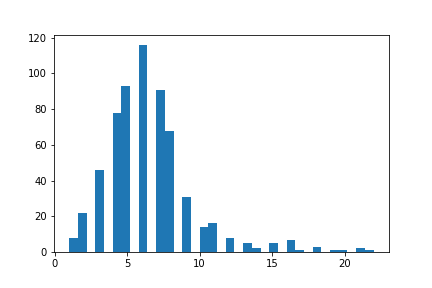
\includegraphics[width=1\linewidth]{predictions_bin15_histogramm}
  \captionof{figure}{Fehlerverteilung}
  \label{fig:hist_bin15}
\end{minipage}
\end{figure}

Im Vergleich zu das Modell vom Versuch Sieben, performt dieses Modell besser, siehe \ref{fig:lage_bin10}. Der Fehler-Score ist etwas geringer, aber im Modell von Versuch Sieben ist das zweite Quintil, sowie der Modus jeweils um eine Einheit niedriger. 

\begin{figure}
\centering
\begin{minipage}{.33\textwidth}
  \centering
  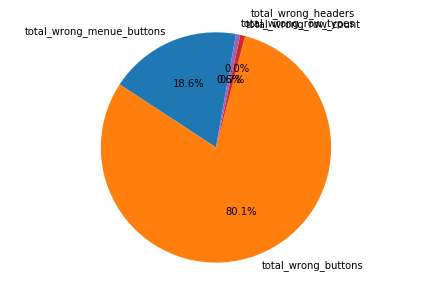
\includegraphics[width=1\linewidth]{predictions_bin15_total_error_types_pie_chart}
  \captionof{figure}{Gesamt}
  \label{fig:fehler_gesamt_bin15}
\end{minipage}%
\begin{minipage}{.33\textwidth}
  \centering
  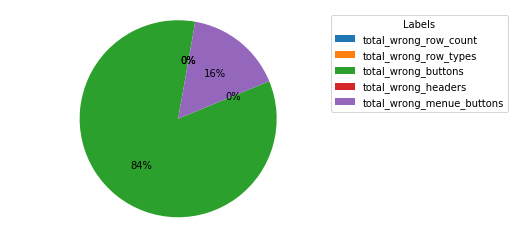
\includegraphics[width=1\linewidth]{predictions_bin15_excluded_p80_error_types_pie_chart}
  \captionof{figure}{Ohne p80}
  \label{fig:fehler_beste80_bin15}
\end{minipage}
\begin{minipage}{.33\textwidth}
  \centering
   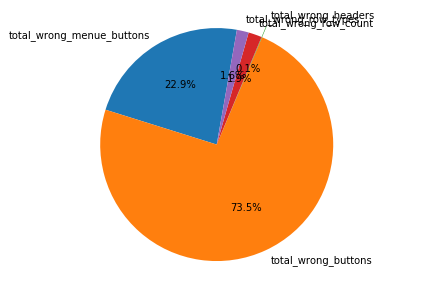
\includegraphics[width=1\linewidth]{predictions_bin15_p80_error_types_pie_chart}
  \captionof{figure}{Nur p80}
  \label{fig:fehler_schlechteste20_bin15}
\end{minipage}
\end{figure}

Die Verteilung der Fehler im letzten Quintil ist ebenso sehr gut; es gab nur 22 mal das Auftreten von falschen Row-Klassifizierungen. Zum Vergleich, im siebten Versuch gab es 174 falsche Klassifizierungen des Row Types.

\begin{figure}[h]
\centering
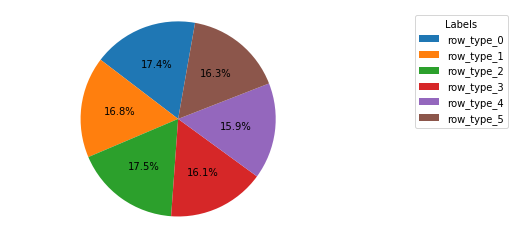
\includegraphics[width=0.3\textwidth]{predictions_bin15_predicted_row_type_distribution}
\caption{Verteilung Row Types}
\label{fig:bin15_row_type}
\end{figure}

Daher ist auch die Verteilung der Row Type sehr gleichmäßig, zu sehen in Abbildung~\ref{fig:bin15_row_type}. 
Der Fehler Score ist gegenüber Versuch Sieben um ca. 18\% gesunken. 
Interessant ist, dass dieses Modell 276\% der Fehler des siebten Versuchs in den Menü-Buttons macht. Außerdem hat es einmal einen falschen Header identifiziert. Bei der Anzahl der falschen Buttons gibt es kaum einen Unterschied zum siebten Modell.

\subsubsection*{Fazit}
Aufgrund der längeren \texttt{CONTEXT\_LENGTH} ist das Ergebnis sehr viel besser geworden. Row-Types werden hier mit am zuverlässigsten erkannt, was wahrscheinlich an der verlängerten \texttt{CONTEXT\_LENGTH} liegt, da das Modell so auf jeden Fall die aktuelle Row als auch die davor gleichzeitig im Speicher haben kann. Leider gibt es Abspriche in der Qualität der Menüs, da hat fast 3 mal so viele Fehler gemacht wie der Vergleich. Die ist aber zu verschmerzen, da Performance der Rows so außerordentlich gut ist. Vielleicht ist das Modell ein bisschen zu einfach um die Komplexität der DSL und der Screenshots ausreichend abzubilden. 

\subsection{13. Trainingsversuch}
%Language: GRU 92 units
%Decoder GRU 386 units

%bin16

\subsubsection*{Einführung}

Hier wird eine vereinfachte Variante des siebten Modells genutzt um zu testen, ob es so besser verallgemeinert.

\subsubsection*{Datenset}

Hier wurde das Datenset aus dem sechsten Trainingsversuch verwendet.

\subsubsection*{Veränderte Parameter}

Sowohl der Sprach- als auch der Decoder-Teil des Modells wurden verkleinert. Die Anzahl der rekurrenten \texttt{Units} sind von 128 auf 92 im Sprach-Teil und von 512 auf 386 im Decoder-Teil reduziert worden.

\begin{verbatim}
Layer (type)                    Output Shape         Param #     Connected to
=============================================================================
input_1 (InputLayer)            (None, 256, 256, 3)  0
_____________________________________________________________________________
input_2 (InputLayer)            (None, 48, 23)       0
_____________________________________________________________________________
sequential_1 (Sequential)       (None, 48, 1024)     104098080   input_1[0][0]
_____________________________________________________________________________
sequential_2 (Sequential)       (None, 48, 92)       83076       input_2[0][0]
_____________________________________________________________________________
concatenate_1 (Concatenate)     (None, 48, 1116)     0           sequential_1[1][0]
                                                                 sequential_2[1][0]
_____________________________________________________________________________
gru_3 (GRU)                     (None, 48, 386)      1740474     concatenate_1[0][0]
_____________________________________________________________________________
gru_4 (GRU)                     (None, 386)          895134      gru_3[0][0]
_____________________________________________________________________________
dense_3 (Dense)                 (None, 23)           8901        gru_4[0][0]


Trainable params: 106,825,665
\end{verbatim}

Diese Änderung sieht man in den Ebenen \texttt{sequential\_2} sowie \texttt{gru\_2} und \texttt{gru\_4}.
Durch die Verkleinerung der RNNs, ist das Modell um knappe zwei Millionen Parameter kleiner geworden.

\subsubsection*{Ergebnis}


Wie in Abbildung~\ref{fig:lage_bin16} zu sehen ist, sind alle Lageparameter schlechter als die bisherigen guten Ergebnisse.

\begin{figure}
\centering
\begin{minipage}{.5\textwidth}
  \centering
  \begin{description}
	\item[Arithmetisches Mittel] $16.71$	
	\item[Geometrisches Mittel] $15.25$
	\item[Harmonisches Mittel] $13.62$
	\item[Quintile] p20: $11$, p40: $15$, p60: $17$, p80: $22$
	\item[Median] $16$
	\item[Modus] $16$
	\item[Vorkommen Modus] $54$
	\item[Gesamt Fehler Score] 10342
	\item[Anzahl Token Testset] 36751 
	\item[Anzahl generierter Token] 36047
	\item[Score pro Token Testset]  0.28
\end{description}
  \captionof{figure}{Lageparameter}
  \label{fig:lage_bin16}
\end{minipage}%
\begin{minipage}{.5\textwidth}
  \centering
  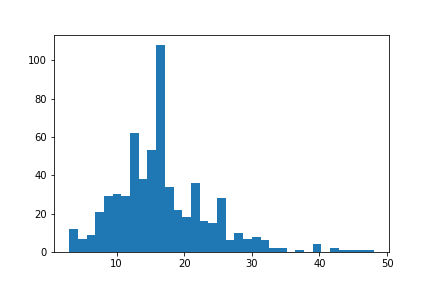
\includegraphics[width=1\linewidth]{predictions_bin16_histogramm}
  \captionof{figure}{Fehlerverteilung}
  \label{fig:hist_bin16}
\end{minipage}
\end{figure}

Im Vergleich der Lageparameter zu dem zehnten Trainingsversuch (LSTM mit mehr Parametern), gibt es hier einen geringeren Fehler-Score. Es ist jedoch zu sehen, an den Abbildungen~\ref{fig:fehler_gesamt_bin16} bis ~\ref{fig:fehler_p80_bin16}, dass dieFehlerverteilung überall gleich ist, egal in welchem Quintil.

\begin{figure}
\centering
\begin{minipage}{.33\textwidth}
  \centering
  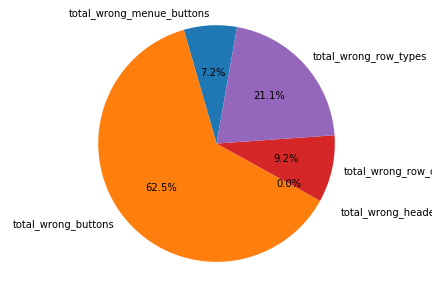
\includegraphics[width=1\linewidth]{predictions_bin16_total_error_types_pie_chart}
  \captionof{figure}{Gesamt}
  \label{fig:fehler_gesamt_bin16}
\end{minipage}%
\begin{minipage}{.33\textwidth}
  \centering
  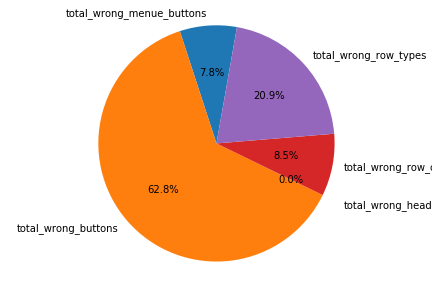
\includegraphics[width=1\linewidth]{predictions_bin16_excluded_p80_error_types_pie_chart}
  \captionof{figure}{Ohne p80}
  \label{fig:fehler_beste80_bin16}
\end{minipage}
\begin{minipage}{.33\textwidth}
  \centering
   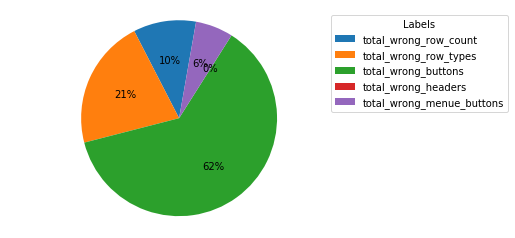
\includegraphics[width=1\linewidth]{predictions_bin16_p80_error_types_pie_chart}
  \captionof{figure}{Nur p80}
  \label{fig:fehler_schlechteste20_bin16}
\end{minipage}
\end{figure}

An der Verteilung der generierten Row Types in Abbildung~\ref{fig:bin16_row_type} erkennt man, dass diese Modell es nicht gelernt hat die Typen zuverlässig zu unterscheiden.

\begin{figure}[h]
\centering
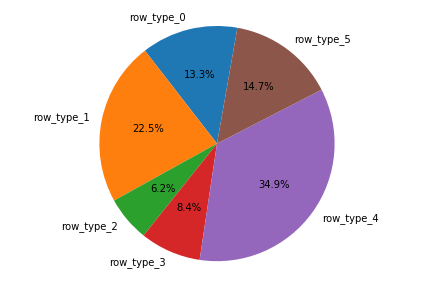
\includegraphics[width=0.3\textwidth]{predictions_bin16_predicted_row_type_distribution}
\caption{Verteilung Row Types}
\label{fig:bin16_row_type}
\end{figure}

\subsubsection*{Fazit}
Durch das Reduzieren der \texttt{Units} der RNNs ist das Modell schlicht zu simpel geworden. Obwohl es die richtige Grammatik lernen konnte - es hat keine Token-Sequenzen erzeugt, die nicht kompiliert werden konnte.


\subsection{Einschub - Funktioniert das original überhaupt?}
Training insegesamt 20 Epochen

\begin{verbatim}


python train.py ../datasets/web/training_features/ ../b
in_orginal/ 1 ../bin_orginal/pix2code.h5 
Epoch 1/10
291/290 [==============================] - 130s 445ms/step - loss: 0.2733
Epoch 2/10
291/290 [==============================] - 126s 434ms/step - loss: 0.2302
Epoch 3/10
291/290 [==============================] - 126s 431ms/step - loss: 0.2251
Epoch 4/10
291/290 [==============================] - 125s 431ms/step - loss: 0.2269
Epoch 5/10
291/290 [==============================] - 125s 431ms/step - loss: 0.2099
Epoch 6/10
291/290 [==============================] - 125s 431ms/step - loss: 0.2140
Epoch 7/10
291/290 [==============================] - 125s 431ms/step - loss: 0.1891
Epoch 8/10
291/290 [==============================] - 125s 431ms/step - loss: 0.1865
Epoch 9/10
291/290 [==============================] - 126s 432ms/step - loss: 0.1880
Epoch 10/10
291/290 [==============================] - 126s 431ms/step - loss: 0.1780
\end{verbatim}
\section{Zusammenfassung}
\section{Fazit}

\bibliographystyle{plain}
\bibliography{sources} 

\end{document}


